
% pdflatex, biber, pdflatex, pdflatex

% for printing add margin
\documentclass[a4paper,titlepage, bibliography=totoc,twoside=semi, BCOR=10mm, openright]{scrbook} 

% for writing 
% \documentclass[a4paper,titlepage, bibliography=totoc]{scrbook} 


% Typesetting
\usepackage[utf8]{inputenc} % enable post-90s text processing
\usepackage[T1]{fontenc}
\usepackage[english]{babel}
\usepackage{microtype}
\usepackage{booktabs}
\usepackage{pgfplotstable} % Required for reading CSV and creating tables
\usepackage{makecell}
\usepackage{dirtytalk}
\usepackage{lmodern} % upgrade default font
\usepackage[sc]{mathpazo} % pretty font for text
\usepackage{pdfpages}
\usepackage{nicefrac}
\usepackage{csquotes}
\usepackage{nameref}
\usepackage{parskip}
\usepackage{caption}
\usepackage{relsize}
\usepackage{listings}
\lstset{
    basicstyle=\ttfamily\footnotesize,
    captionpos=b,
    breaklines=false,
    backgroundcolor=\color{backcolour},   
    commentstyle=\color{codegreen},
    keywordstyle=\color{magenta},
    numberstyle=\tiny\color{codegray},
    stringstyle=\color{codepurple},
    basicstyle=\ttfamily\footnotesize,
    numbers=left, 
            framexleftmargin=4pt,
}
\definecolor{codegreen}{rgb}{0,0.6,0}
\definecolor{codegray}{rgb}{0.5,0.5,0.5}
\definecolor{codepurple}{rgb}{0.58,0,0.82}
\definecolor{backcolour}{rgb}{0.95,0.95,0.92}

\usepackage{float}
\newfloat{lstfloat}{t}{lop}
\floatname{lstfloat}{Listing}



% Links and Metadata
\usepackage[
  colorlinks,
  citecolor = DarkBlue,  
  linkcolor = DarkBlue,
  urlcolor = DarkBlue
]{hyperref}
\usepackage{bookmark}


% Math & Symbols
\usepackage{mathtools}
\usepackage{amssymb}
\usepackage{amsbsy}
\usepackage{amsmath}
\usepackage{amsthm}
\usepackage{stmaryrd}

\usepackage{braket}
\usepackage{cool}
\usepackage{accents}
\usepackage{stackengine}


\usepackage{bm}
\usepackage{nicefrac}
\usepackage[super]{nth}
\usepackage{hyphenat}

\usepackage{thmtools}
\usepackage{enumitem}
\usepackage[export]{adjustbox}
\usepackage{graphicx}

% Utilities
\usepackage{lipsum} 
\usepackage{varioref}
\usepackage[nameinlink,noabbrev]{cleveref}
\creflabelformat{equation}{#2\textup{#1}#3}
\renewcommand{\cref}{\Cref} % uppercase for all crefs

\usepackage{subcaption} % format \cref: figure 1.1 (i)
\captionsetup[figure]{font=small}
\renewcommand\thesubfigure{ (\roman{subfigure})} 

% Colors
\usepackage[svgnames]{xcolor}
% https://s3.amazonaws.com/edwardtufte.com/colorblind_palette.png

\definecolor{myorange}{RGB}{230,159,0} 
\definecolor{myblue}{RGB}{55,126,184}
\definecolor{mygreen}{RGB}{77,175,74}
\definecolor{myred}{RGB}{228,26,28}
\definecolor{mypink}{RGB}{204,121,167}
\definecolor{mygray}{rgb}{0.66, 0.66, 0.66}

%%%%%%%%%%%%%%%%%%%%%%%%%%%%%%%%%%%%%%%%%%%%%%%%%%%%%%%%%%%%%%%%
% Environments
\usepackage{array}
\usepackage{blkarray}  % cool blockarrays
\usepackage[most]{tcolorbox}

% A nice way to comment the text is given by the following:
\usepackage{todonotes}
\setlength{\marginparwidth}{3cm}
\usepackage{marginnote}

\usepackage{tikz}
\usetikzlibrary{automata,arrows,positioning,calc,fit,backgrounds,shapes.geometric}
%\tikzset{snake arrow/.style={->,decorate, decoration={snake, amplitude=.4mm,segment length=2mm, post length=1mm}}}
%\tikzset{snake line/.style={decorate, decoration={snake, amplitude=.4mm,segment length=2mm}}}

\usepackage{algorithm}
\usepackage{algpseudocode}
\algnewcommand{\LineComment}[1]{\State \(\triangleright\) #1}

\usepackage{float}

\usepackage{hyphenat}
\hyphenation{non-termination non-deterministic non-probabilistic}

\usepackage{pgfplots}
\pgfplotsset{compat=1.17}
\usepackage{hyperref}
\hypersetup{
    colorlinks=true,    % Enables coloring of links
    linkcolor=black,    % Sets the color for internal links (like \ref)
    citecolor=black,    % Sets the color for citation links (like \cite)
    urlcolor=black      % Sets the color for URLs
}
% abs, norm
\DeclarePairedDelimiter\abs{\lvert}{\rvert}%
\DeclarePairedDelimiter\norm{\lVert}{\rVert}%



%%%%%%%%%%%%%% Theorem boxes 
\tcbuselibrary{theorems}
\tcbset{boxrule=0pt,toprule=1pt}

\newtheoremstyle{theoremdd}% name of the style to be used
  {0.5\baselineskip}% measure of space to leave above the theorem. E.g.: 3pt
  {0.5\baselineskip}% measure of space to leave below the theorem. E.g.: 3pt
  {}% name of font to use in the body of the theorem
  {}% measure of space to indent
  {\bfseries}% name of head font
  {:}% punctuation between head and body
  {.5em}% space after theorem head; " " = normal interword space
  {}
\theoremstyle{theoremdd}

\newcommand{\newcooltheorem}[5]{%
  \makeatletter
  \Crefname{tcb@cnt@#1}{#2}{#2s}%
  %\Crefname{tcb@cnt@#1}{#2}
  \makeatother
  \newtcbtheorem[list inside=#1, number within=chapter]{#1}{#2}{
    % if number within section: add thesection to enumthm cref
    % Example Frame Start
    empty,% Empty previously set parameters
    % Attaching a box requires an overlay
    attach boxed title to top left,
    % Ensures proper line breaking in longer titles
    minipage boxed title,
    % (boxed title style requires an overlay)
    boxed title style={empty,size=minimal, 
    toprule=0pt,top=4pt,left=3mm},
    % title formatting
    coltitle=black,fonttitle=\scshape,description font=\normalfont\bfseries\sffamily, separator sign={. },
    % spacing
    before=\par\medskip\noindent,parbox=false,boxsep=0pt,left=3mm,right=3mm,top=5pt,breakable,pad at break=0mm,
    before upper=\csname @totalleftmargin\endcsname0pt, % Use instead of parbox=true. 
    %This ensures parskip is inherited by box.
    %
    % Handles box when it exists on one page only
    overlay unbroken={\draw[#4,line width=.5pt] ([xshift=-0pt]title.north west) -- ([xshift=-0pt]frame.south west); 
    \begin{scope}[on background layer]
      \fill[#5] 
      (frame.south west) -- 
      (title.north west) -- 
      ([xshift=3mm]title.north east) --
      (frame.south east);
      % \node (box) [fill=blue!20, fit = {(frame.south west),
      % (title.north west),
      % (title.north east),
      % (frame.south east)}{};
    \end{scope}[on background layer]
    },
    % Handles multipage box: first page
    overlay first={\draw[#4,line width=.5pt] ([xshift=-0pt]title.north west) -- ([xshift=-0pt,yshift=-3mm]frame.south west); 
    \begin{scope}[on background layer]
      \fill[#5] 
      ([yshift=-3mm]frame.south west) -- 
      (title.north west) -- 
      ([xshift=3mm]title.north east) --
      ([yshift=-3mm]frame.south east);
      \end{scope}[on background layer]
    },
    % Handles multipage box: middle page
    overlay middle={\draw[#4,line width=.5pt] ([xshift=-0pt, yshift=3mm]frame.north west) -- ([xshift=-0pt]frame.south west); 
    \begin{scope}[on background layer]
      \fill[#5] 
      (frame.south west) -- 
      ([yshift=3mm]frame.north west) -- 
      ([yshift=3mm]frame.north east) --
      (frame.south east);
      \end{scope}[on background layer]
    },
    % Handles multipage box: last page
    overlay last={\draw[#4,line width=.5pt] ([xshift=-0pt, yshift=3mm]frame.north west) -- ([xshift=-0pt]frame.south west); 
    \begin{scope}[on background layer]
      \fill[#5] 
      (frame.south west) -- 
      ([yshift=3mm]frame.north west) -- 
      ([yshift=3mm]frame.north east) --
      (frame.south east);
      \end{scope}[on background layer]
      },%
    }{#3}%
}%

\newcooltheorem{mydefinition}{Definition}{def}{myblue}{white} %{skyblue!70!black}   % todo rot/orange (?)
\newcooltheorem{myexample}{Example}{ex}{mygreen}{mygreen, opacity=0.07} %{bluishgreen!70!black}      % todo grün
\newcooltheorem{mytheorem}{Theorem}{theo}{myred}{white} %{reddishpurple!70!black}  %todo blau
\newcooltheorem{mylemma}{Lemma}{theo}{myred}{white}
\newcooltheorem{myproposition}{Proposition}{theo}{myred}{white}
\newcooltheorem{mycorollary}{Corollary}{theo}{myred}{white} 
\newcooltheorem{myproblem}{Problem}{prob}{mypink}{mypink, opacity=0.1}

\theoremstyle{remark}
\newtheorem{remark}{Remark}[chapter]

% footnotemarks inside align
\makeatletter
\let\original@footnotemark\footnotemark
\newcommand{\align@footnotemark}{%
  \ifmeasuring@
    \chardef\@tempfn=\value{footnote}%
    \original@footnotemark
    \setcounter{footnote}{\@tempfn}%
  \else
    \iffirstchoice@
      \original@footnotemark
    \fi
  \fi}
\pretocmd{\start@align}{\let\footnotemark\align@footnotemark}{}{}
\makeatother

\newcommand{\defeq}{\vcentcolon=}
\newcommand{\eqdef}{=\vcentcolon}
\newcommand{\N}{\mathbb{N}}
\newcommand{\R}{\mathbb{R}}
\newcommand{\Z}{\mathbb{Z}}
\newcommand{\Q}{\mathbb{Q}}
\newcommand{\C}{\mathbb{C}}
\newcommand{\Pred}{\operatorname{Pred}}
\newcommand{\Succ}{\operatorname{Succ}}
\newcommand{\Reach}{\operatorname{Reach}}
\newcommand{\Cone}{\operatorname{Cone}}
\newcommand{\satr}{\operatorname{satr}}
\newcommand{\watr}{\operatorname{watr}}
\newcommand{\ASReach}{\operatorname{ASReach}}
\renewcommand{\Pr}{\operatorname{Pr}}
\newcommand\CC{
    C++
}
\renewcommand{\set}[1]{\mathopen{}\left\{\;\!#1\;\!\right\}\mathclose{}}

\def\until{\mathsf{U}}

\newcommand{\mycomment}[2][]{\todo[size=\footnotesize, #1]{#2}}
\newcommand{\mytodo}[2][]{\todo[color=red, size=\footnotesize, #1]{TODO: #2}}

% multiline stuff for algpseudocode
\iffalse
\newcommand\CONDITION[2]%
   {\begin{tabular}[t]{@{}l@{}}#1#2\end{tabular}}
\algdef{SE}[WHILE]{While}{EndWhile}[1]%
   {\algorithmicwhile\ \CONDITION{#1}{\ \algorithmicdo}}%
   {\algorithmicend\ \algorithmicwhile}
\algdef{SE}[FOR]{For}{EndFor}[1]%
   {\algorithmicfor\ \CONDITION{#1}{\ \algorithmicdo}}%
   {\algorithmicend\ \algorithmicfor}
\algdef{S}[FOR]{ForAll}[1]%
   {\algorithmicforall\ \CONDITION{#1}{\ \algorithmicdo}}
\algdef{SE}[REPEAT]{Repeat}{Until}%
   {\algorithmicrepeat}[1]%
   {\algorithmicuntil\ \CONDITION{#1}{}}
\algdef{SE}[IF]{If}{EndIf}[1]%
   {\algorithmicif\ \CONDITION{#1}{\ \algorithmicthen}}%
   {\algorithmicend\ \algorithmicif}
\algdef{C}[IF]{IF}{ElsIf}[1]%
   {\algorithmicelse\ \algorithmicif\ \CONDITION{#1}{\ \algorithmicthen}}
   
\makeatletter
\ifthenelse{\equal{\ALG@noend}{t}}%
   {\algtext*{EndWhile}%
    \algtext*{EndFor}%
    \algtext*{EndLoop}%
    \algtext*{EndIf}%
   }{}%
\makeatother
\fi


\setlength\parindent{0pt} % noindent

\begin{document}
%\listoftodos

\frontmatter
\makeatletter
\begin{titlepage}

  \centering
  \vspace*{1cm}
  {\huge\textbf{\textsc{Bachelors's Thesis}}} \\ % or Bachelor's
  \vspace{0.5cm}
  {\Huge{}
  \rule{\linewidth}{0.75pt} %
  \vspace*{-1.25cm}

  {\textbf{Model Checking Stochastic Games\\with Storm}} \\
  \vspace*{0.2cm} \rule{\linewidth}{0.75pt}} \\

  \vspace{1.5cm}
  {\large{}\textit{by}} \\
  \vspace{0.2cm}
  {\Large{}Jannik Hiller} \\ %  replace by author's Name
  \vspace{2cm}

  \textit{\nth{1} Examiner:} \\
  Prof. Dr. Ir. Dr. h.c. Joost-Pieter Katoen\\[1em]
  \textit{\nth{2} Examiner:} \\
  Apl. Prof. Dr. Thomas Noll\\[1em]
  \textit{Supervisor:} \\
  Dr. Tim Quatmann, Hannah Mertens
  \vspace{3em}
    
  \textit{The present work was submitted to:} \\
  Chair for Software Modeling and Verification 
  \\RWTH Aachen
  \vspace{1.5cm}

  \@date
\end{titlepage}
\makeatother


%\includepdf{Formular_Eidesstattliche_Versicherung.pdf}

\chapter*{\centering Abstract}
Stochastic multiplayer games (SMGs) are a formalism for modeling systems that incorporate stochastic behavior and competitive or cooperative interactions among multiple players. A fundamental question in this setting is almost-sure reachability, which asks whether a set of target states can be reached with probability one regardless of the strategies chosen by other players.
This thesis provides a formal definition and correctness proof for an algorithm solving almost-sure reachability in SMGs, with a run time complexity of $\Theta(nm)$. It is based on a nested fix-point calculation. While similar algorithms are implemented in existing model checking tools such as PRISM-games, we optimized it by adapting the inner loop to work in layers. The algorithm is implemented in the Storm model checker, achieving significant performance improvements over PRISM-games, with speedups ranging from 5x to 25x, particularly for smaller input sizes. This implementation lays the groundwork for extending Storm with quantitative model-checking of stochastic multiplayer games in the future.

\clearpage
\begingroup
\pagestyle{empty}
\renewcommand*{\chapterpagestyle}{empty}
\tableofcontents
\clearpage
\endgroup

\addtocontents{toc}{\protect\setcounter{tocdepth}{1}}
\setcounter{secnumdepth}{2}

\cleardoublepage

\mainmatter
\chapter{Introduction}
\label{chap:intro}

\section{Motivation and Context}
Formal verification of systems is of critical importance, particularly in safety-critical applications. Examples include autonomous driving, energy management, and communication protocols, where even minor failures can lead to catastrophic consequences.

Many of these applications exhibit both nondeterministic and probabilistic behavior. Such systems can be naturally modeled using Markov Decision Processes (MDPs) \cite{puterman_markov_2014}. MDPs provide a formal framework to capture systems with stochastic transitions and nondeterministic choices.

MDPs can be extended to accommodate multiple actors (players), where each player controls a subset of the nondeterministic choices. The resulting formalism is referred to as a \textit{Stochastic Multiplayer Game (SMG)}. SMGs are a powerful model for systems that involve competition or collaboration between agents, alongside probabilistic dynamics.

SMGs have a wide range of practical applications, including:
\begin{itemize}
    \item \textbf{Security and communication protocols}: Ensuring robustness in adversarial environments \cite{kremer_game-based_2001, park_lisp_2004, perrig_spins_2001, van_der_hoek_model_2003, wu_model_2005}.
    \item \textbf{Robotics and pursuit-evasion games}: Modeling strategies for multiple interacting robots \cite{hespanha_multiple-agent_1999}.
    \item \textbf{Energy markets}: Simulating competition and cooperation in future energy systems \cite{hildmann_influence_2011, chen_automatic_2013}.
    \item \textbf{Sensor networks}: Optimizing collective decision-making processes in distributed systems \cite{saffre_host_2012, chen_automatic_2013}.
\end{itemize}

\textbf{Qualitative reachability} is a fundamental objective in the analysis of SMGs. It focuses on determining whether a player is able to enforce reaching a target set of states with probability $0$ or $1$, regardless of the strategies employed by the other players. Reachability serves as a crucial preprocessing step in established model checkers for stochastic systems, such as Storm \cite{hensel_probabilistic_2020} and PRISM-games \cite{chen_automatic_2013}.

In this thesis, we present an algorithm for qualitative reachability. Although similar algorithms are implemented in existing model checking tools such as PRISM-games, this thesis extends prior work by providing a detailed formalization and a rigorous correctness proof. The algorithm can serve as a reference for future implementations.

The algorithm is based on a fixed-point calculation. The main idea is to maintain a working set by repeatedly calculating the set of states from which a player can reach a target set with a non-zero probability, while disregarding the states from which the adversarial players can enforce leaving the working set with non-zero probability. In each iteration, more such states are determined and subsequently disregarded when computing the next working set. Eventually the working set only contains states from which the player can reach the target set with probability $1$.

We also introduce an improvement over the implementation in PRISM-games. To compute the set of states from which the target set can be reached with a non-zero probability, PRISM-games repeatedly iterates over all states. Our approach improves upon this by working in layers of states, each of which consists of predecessor states of the previous layer.

\section{Related Work}
Several works have addressed the verification of SMGs and related models.

Chatterjee et al. \cite{chatterjee_simple_2003} focus on qualitative properties expressed in $\omega$-regular specifications within the context of two-player stochastic games. They propose an efficient translation of these games into non-stochastic parity games, enabling the use of established algorithms for analysis. For the specific case of Markov Decision Processes (MDPs) with Büchi objectives, where the goal is to reach a target set infinitely often---a stricter condition than simple reachability---they present an algorithm with a time complexity of $O(m \sqrt{m})$.

In subsequent work, Chatterjee et al. \cite{chatterjee_on2_2011} describes an $O(n^2)$ algorithm for Büchi objectives in alternating games. They utilize a dynamic programming approach and their method is further extended to stochastic alternating games, which are a subclass of stochastic multi-player games (SMGs), providing an algorithm for almost-sure reachability with $O(nm)$ runtime.

Chen et al. \cite{chen_automatic_2013, chen_automatic_2013-1} presented methods for model checking SMGs in the probabilistic model checker PRISM-games\cite{lahiri_prism-games_2020}. Their work focuses on quantitative properties and uses value iteration as the main computational technique. For qualitative reachability, PRISM-games performs a preprocessing step, but the algorithm is not formally described. PRISM-games is used as a baseline implementation for our experiments in chapter~\ref{chap:eval}.

Hahn et al. \cite{chaudhuri_simple_2016} present an algorithm for qualitative parity objectives in stochastic multi-player games (SMGs) with a runtime of $O(n^{O(\sqrt{n})})$. Their work adapts an algorithm originally designed for non-stochastic two-player games to the SMG setting. Additionally, their definitions of strong and weak attractors served as a foundation for the development of our algorithm.


\section{Contributions}
This thesis makes several significant contributions to the field of model checking stochastic games:

\begin{itemize}
    \item We provide a formal definition of an algorithm for computing positive and almost-sure reachability in stochastic games with a runtime of $\Theta(nm)$. It is based on the concept of strong- and weak-attractors by Hahn et\ al. \cite{chaudhuri_simple_2016}. While almost-sure reachability is well-studied, existing literature lacked a clear and rigorous formalization of the algorithm. Such a formalization aids in future implementations of model-checking algorithms for SMGs.
    \item We prove the correctness of the proposed algorithm. This step is crucial to ensure that the algorithms used for SMG model checking are both reliable and robust.
    \item We implement a high-performance version of the algorithm for the probabilistic model checker Storm. Since almost-sure reachability can also serve as a preprocessing step for quantitative model checking, our implementation is a foundational building block for further SMG model-checking developments using Storm.
    \item An experimental evaluation of our implementation demonstrates significant efficiency, outperforming the PRISM model checker by at least a factor of 5, with particularly notable speedups for smaller input sizes.
\end{itemize}


\section{Structure of the Thesis}
\begin{itemize}
    \item \textbf{Chapter \ref{chap:intro}: \nameref{chap:intro}}.
    This chapter provides the motivation and context for the thesis. It introduces the problem, outlines the contributions, and gives an overview of the thesis structure.
    
    \item \textbf{Chapter \ref{chap:prelim}: \nameref{chap:prelim}}.  
    This chapter lays the theoretical groundwork necessary for the thesis. It covers the essential mathematical background in probability theory and provides formal definitions of stochastic games, including qualitative reachability.

    \item \textbf{Chapter \ref{chap:reach}: \nameref{chap:reach}}.
    This chapter constitutes the main theoretical contribution of the thesis. It introduces the concepts of strong and weak attractors and proves their equivalence to reachability and almost-sure reachability. It also presents an algorithm for computing strong and weak attractors and analyzes its worst-case runtime.

    \item \textbf{Chapter \ref{chap:eval}: \nameref{chap:eval}}.
    This chapter evaluates the performance and scalability of the implemented algorithm. The algorithm's performance is compared with the model checker PRISM on several real-world and synthetic scenarios.

    \item \textbf{Chapter \ref{chap:conc}: \nameref{chap:conc}}.
    The final chapter summarizes the findings of the thesis and discusses possible directions for future research.
\end{itemize}

\chapter{Preliminaries}
\label{chap:prelim}
\section{Mathematical Background}
This section introduces essential notation and mathematical concepts. 

\subsection{Sets}
A \textit{set} is a collection of elements, usually denoted by capital letters (e.g., $A$, $S$, $X$). Elements within sets are represented by lower-case letters.

The following special sets are used throughout this thesis:
\begin{itemize}
    \item The empty set: $\emptyset$,
    \item The set of natural numbers: $\mathbb{N} \defeq \{0, 1, 2, \dots\}$,
    \item The set of natural numbers up to $n$: $\underline{n}\defeq\set{i\in\N\mid 0\leq i\leq n}$,
    \item The set of integers: $\mathbb{Z} \defeq \{\dots, -2, -1, 0, 1, 2, \dots\}$,
    \item The set of real numbers: $\mathbb{R}$,
    \item Intervals: $[a, b] \defeq \{x \in \mathbb{R} \mid a \leq x \leq b\}$,
    \item The power set: $2^A$, which is the set of all subsets of $A$
\end{itemize}

\subsection{Functions}
A \textit{function} is a mapping from each element of a set $X$ (called the \textit{domain}) to a single element in a set $Y$ (called the \textit{codomain}). Functions are typically denoted by lower-case letters, such as $f$. 

The function $f$ from $X$ to $Y$ is denoted as:
\[
f: X \to Y
\]

For an element $x \in X$, the function’s value at $x$ is denoted by $f(x) \in Y$. A function can also be defined explicitly, for example:
\[
f(x) \defeq x^2 + 1
\]
A \textit{partial function} has the special codomain element $\bot$. If $f(x) = \bot$ for some $x$, the function is considered undefined at $x$.

In some cases, standard naming conventions for sets and functions are adjusted for clarity, especially when commonly accepted alternative symbols exist.

\subsection{Discrete Probability Distributions}
The following definitions on probability are based on Cramer \cite[Chapter 2]{cramer_statistik_2007}. Let $\Omega$ be a finite or countably infinite set, referred to as the \textit{sample space}. Define a function $p: \Omega \to [0, 1]$ such that:
\[
\sum_{\omega \in \Omega} p(\omega) = 1
\]

A \textit{discrete probability distribution} is a function $\Pr: 2^\Omega \to [0, 1]$ defined as:
\[
\Pr(A) \defeq \sum_{\omega \in A} p(\omega) \quad \text{for} \quad A \in 2^\Omega
\]

The function $p$ is called the \textit{probability mass function} of $\Pr$. For a single element $\omega\in\Omega$, the notation $\Pr(\omega)\defeq\Pr(\set{\omega})$ can be use as a shorthand. A probability distribution $\Pr$ is called \textit{deterministic} if $p(\omega)=1$ for some $\omega\in\Omega$.

The set $\mathcal{D}(\Omega)$ represents all discrete probability distributions over the sample space $\Omega$. The \textit{Dirac distribution} for an element $\omega\in\Omega$ is defined by \[
\delta_\omega(A)\defeq\begin{cases}
    1 & \text{if } \omega \in A\\
    0 & \text{otherwise}\\
\end{cases}\]

\subsection{Probability spaces}
Not all probabilistic events that we are interested in are subsets of countable sets. For example, later in this thesis, we want to assign probabilities to subsets of the set of all infinite paths in a graph, which is an uncountable set. Therefore, we introduce \textit{probability spaces}.
\begin{mydefinition}{Probability space}{def:prob}
A probability space is a tuple $(\Omega, \mathcal{F}, \mu)$, where:
\begin{itemize}
    \item $\Omega \neq \emptyset$ is a (possibly uncountable) sample space,
    \item $\mathcal{F} \subseteq 2^\Omega$ is a \textit{event space}, 
    \item $\mu: \mathcal{F} \to [0, 1]$ is a probability measure,
\end{itemize}
and it holds that: 
\begin{enumerate}
    \item $\Omega \in \mathcal{F}$,
    \item $\mathcal{F}$ is closed under complementation: $\forall A \in \mathcal{F},\quad A^c = \Omega \setminus A \in \mathcal{F}$, 
    \item $\mathcal{F}$ is closed under countable union: $\forall A_0, A_1, \dots \in \mathcal{F}, \quad \bigcup_{i \in \mathbb{N}} A_i \in \mathcal{F}$,
    \item $\mu(\Omega) = 1$,
    \item $\mu$ is \textit{countably additive}: For any disjoint sets $A_0, A_1, \dots \in \mathcal{F}$, where $A_i \cap A_j = \emptyset$ for $i \neq j$, it holds that:
    \[
    \mu\left(\bigcup_{i \in \mathbb{N}} A_i\right) = \sum_{i \in \mathbb{N}} \mu(A_i).
    \]
\end{enumerate}
An event space $\mathcal{F}$ is called a \textit{$\sigma$-algebra} if conditions 1–3 are satisfied, and a probability function $\mu$ on a $\sigma$-algebra $\mathcal{F}$ is called a \textit{probability measure} if conditions 4 and 5 are satisfied.

Let $\mathcal{C} \subseteq 2^\Omega$ be a collection of sets. The least $\sigma$-algebra containing $\mathcal{C}$ is called the \textit{$\sigma$-algebra generated by $\mathcal{C}$}, denoted by $\sigma(\mathcal{C})$. It exists, is unique, and corresponds to the closure of $\mathcal{C}$ under conditions 1–3. 
\end{mydefinition}


\subsection{Languages}
The following definitions are taken from Staiger \cite{staiger_omega-languages_1997}. Let $\Sigma$ be a finite set of symbols, called the \textit{alphabet}. A \textit{word} over $\Sigma$ is a finite sequence of elements $a_0a_1\ldots$, where $a_i \in \Sigma$ for all $i \geq 0$. The empty word is denoted by $\varepsilon$. Sets of words are referred to as \textit{languages}. Given languages $L$ and $L'$ over $\Sigma$, the following operators are defined:
\begin{itemize}
    \item Concatenation: $LL' \defeq \{ ww' \mid w \in L, w' \in L' \}$
    \item $n$-fold concatenation: $L^n \defeq \underbrace{L L \ldots L}_{n \text{ times}} = \{ w_0w_1\ldots w_n \mid w_i \in L, i \in \underline{n} \},\quad n\in\N$
    \item Kleene star: $L^\ast \defeq \bigcup_{i \in \mathbb{N}} L^i$
    \item Infinite concatenation: $L^\omega \defeq \{ w_0w_1\ldots \mid w_i \in L, i \in \mathbb{N} \}$ (where $L \neq \emptyset$ and $\varepsilon\notin L$). Concatenation of $L^\omega$ with $L'$ on the right ($L^\omega L'$) is undefined.
\end{itemize}

Correspondingly, the set of all finite words over an alphabet $\Sigma$ is $\Sigma^\ast$, the set of all infinite words is $\Sigma^\omega$. A language is called \textit{regular} if it can be produced by union, concatenation, and application of the Kleene star on languages of the form $\set{\varepsilon}$, $\set{a}$ (where $a\in\Sigma$) and the empty set. A language is called \textit{$\omega$-regular} if it can be produced by concatenation of a regular language and a $\omega$-regular language, the union of two $\omega$-regular languages, and infinite concatenation of a regular language not containing the empty word.




\section{Stochastic Multi-Player Games}
This thesis uses the definition by Chen et al. \cite[Definition 1]{chen_automatic_2013}. In a stochastic multi-player game (SMG), the system is represented as a finite graph. Each vertex, referred to as \textit{state}, corresponds to a player and has an associated set of available actions. The game proceeds as follows: In each round, the active player (i.e., the player associated with the current state) selects an action at the current vertex. Subsequently, the next state is chosen probabilistically based on a distribution determined by the current state and the chosen action.
\vspace{2mm}

\begin{mydefinition}{Stochastic Multi-Player Game (SMG)}{def:smg}
A SMG $\mathcal{G}$ is a tuple $(\Pi, S, A, (S_i)_{i\in\Pi}, \Delta, AP, \chi)$, where:
\begin{itemize}
    \item $\Pi$ is a finite set of players,
    \item $S$ is a finite, non-empty set of states,
    \item $A$ is a finite, non-empty set of actions,
    \item $(S_i)_{i\in\Pi}$ is a partition of $S$,
    \item $\Delta: S \times A \to \mathcal{D}(S) \cup \{\bot\}$ is a partial transition function,
    \item $AP$ is a finite set of atomic propositions,
    \item $\chi: S \to 2^{AP}$ is a labelling function.
\end{itemize}
\end{mydefinition}

For each state $s \in S$, let $A(s) \defeq \set{a \in A \mid \Delta(s, a) \neq \bot}$ denote the set of available actions in state $s$. The current player, meaning the player $i \in \Pi$ such that $s \in S_i$, selects an action $a \in A(s)$, and the next state is drawn according to $\Delta(s, a)$.

The \textit{number of transitions} of an SMG is defined as $|\Delta|\defeq |\set{(s, a)\mid a\in A(s)}|$. In contexts where the meaning is clear, we will sometimes refer to the number of states and transitions as $n\defeq |S|$ and $m\defeq |\Delta|$, respectively. A finite or infinite sequence of states and actions $s_0a_0s_1a_1...\in (SA)^\ast S\cup(SA)^\omega$ is called a path. It is called \textit{valid} if $a_i\in A(s_i)$ and $\Delta(s_i, a_i)(s_{i+1})>0$ . Finite paths are usually denoted by $\lambda=s_0a_0s_1a_1...$, infinite paths by $\omega$. The sequence of states in a path $\lambda$ is denoted by $st_\lambda\defeq s_0s_1...$, the set of all infinite paths is $\Omega_\mathcal{G}$ and the set of infinite paths starting in a state $s'\in S$ is $\Omega_{\mathcal{G},s'}$.

Throughout this work, we assume that every state has at least one successor, i.e., $A(s) \neq \emptyset$ for all $s \in S$. This assumption does not reduce the expressiveness of the model, as terminal behavior can be emulated by introducing sink states. The purpose of this assumption is that all paths in the game are infinite.
\begin{figure}[t]
    \centering
\begin{tikzpicture}[>=stealth, node distance=3cm, every node/.style={font=\small}]

% Nodes
\node[draw, minimum size=1cm, shape=rectangle] (S1) {$s_1$};
\node[draw, minimum size=1cm, regular polygon,regular polygon sides=3,right= 5cm of S1] (S2) {$s_2$};
\node[draw, minimum size=1cm, shape=circle, below= 3cm of $(S1)!0.5!(S2)$] (S3) {$s_3$};

\draw[-] (S1) -- node[below left, pos=0.5] {$a$} ($(S1)!0.5!(S3)$);
\filldraw[black] ($(S1)!0.5!(S3)$) circle (2pt); % Dot at split point
\draw[->] ($(S1)!0.5!(S3)$) -- node[below left, pos=0.5] {$\frac{2}{3}$} (S3);
\draw[->] ($(S1)!0.5!(S3)$) -> node[below, pos=0.75] {$\frac{1}{3}$} (S2);
\draw[-] (S2) -- node[below right, pos=0.5] {$a$} ($(S2)!0.5!(S3)$);
\filldraw[black] ($(S2)!0.5!(S3)$) circle (2pt); % Dot at split point
\draw[->] ($(S2)!0.5!(S3)$) -- node[below right, pos=0.5] {$\frac{1}{2}$} (S3);
\draw[->] ($(S2)!0.5!(S3)$) -- node[below, pos=0.75] {$\frac{1}{2}$} (S1);

\draw[->] (S1) to[bend left=30] node[above, pos=0.25] {$b$} 
node[above, pos=0.75] {$1$} coordinate[pos=0.5] (S1S2) (S2);
\filldraw[black] (S1S2) circle (2pt); % Dot halfway along the curve

\draw[->] (S2) -> node[above, pos=0.25] {$b$} node[above, pos=0.75] {$1$} coordinate[pos=0.5] (S2S1) (S1);
\filldraw[black] (S2S1) circle (2pt); % Dot halfway along the curve

\draw[->] (S3) edge[loop below]
coordinate[pos=0.5] (S3S3)
node[right, pos=0.2] {$c$}
node[left, pos=0.8] {$1$} (S3);
\filldraw[black] (S3S3) circle (2pt); % Dot halfway along the curve

\end{tikzpicture}
    \caption{Example of a SMG with three players and three actions}
    \label{fig:example_game_01}
\end{figure}

\begin{myexample}{Simple SMG}{ex:simple_smg}
Figure~\ref{fig:example_game_01} shows an example of a SMG. It has three players: \textit{square}, \textit{triangle} and \textit{circle}. The outgoing edges correspond to the available action, e.g., $A(s_1)=\set{a, b}$. The multiple ends of each edge represent the states that have a non-zero probability according to the transition function $\Delta$. They are labeled with their probabilities. E.g., $\Delta(s_1, a)(s_2)=\frac{1}{3}$ and $\Delta(s_1, a)(s_3)=\frac{2}{3}$.
\end{myexample}
Note that another well-studied model related to SMGs is that of \textit{Markov Decision Processes} (MDPs). MDPs describe systems with non-deterministic and probabilistic behavior controlled by a single agent. They are equivalent to stochastic multiplayer games (SMGs) with $|\Pi| = 1$.


\subsection{Strategies}\label{def:strat}

To reason about nondeterministic behavior of multiple players, it is useful to introduce \textit{strategies}. A strategy is a function that describes the decision a player makes in each step.
\begin{mydefinition}{Strategy}{def:strat}
Let $\mathcal{G}=(\Pi, S, A, (S_i)_{i\in\Pi}, \Delta, AP, \chi)$ be a SMG. A strategy for a player $i\in\Pi$ is a function $\sigma_i: (SA)^\ast S_i\rightarrow\mathcal{D}(A)$, 
where $\sigma_i(\lambda s)$ is a probability distribution over $A(s)$ and $\lambda s\in (SA)^\ast S_i$.
\end{mydefinition}
A strategy $\sigma_i$ is called \textit{memoryless} if it is path-independent, this means $\sigma_i(\lambda s) = \sigma_i(\lambda' s)$ for all $\lambda, \lambda'\in (SA)^\ast, s\in S_i$ and is called \textit{deterministic} if $\sigma_i(\lambda s)$ is deterministic.

$\Sigma_i$ denotes the set of all strategies for player $i\in\Pi$. A \textit{strategy profile} $\sigma=\sigma_0,...,\sigma_{|\Pi|-1}$ contains a strategy for each player.

\subsection{Outcomes of Strategies}\label{sec:prop_measure}
An SMG $\mathcal{G}$ paired with a strategy profile becomes a purely probabilistic process, as all non-deterministic choices of players are determined. To formalize this, we introduce a $\sigma$-algebra over the paths in $\mathcal{G}$, following the definitions of Chatterjee \cite[Section 2.2.2]{chatterjee_stochastic_2007}.

Given a finite path $\lambda = s_0 a_0 s_1 a_1 \dots s_n$, the \textit{cone} of $\lambda$ is the set 
\[
\Cone(\lambda) \defeq \set{ s'_0 a'_0 s'_1 \dots \in \Omega_\mathcal{G} \mid s_i = s'_i \text{ and } a_i = a'_i, \; i \in \underline{n}}
\]
of infinite paths that have $\lambda$ as their prefix. Let $\mathcal{U} \defeq \left\{ \text{Cone}(\lambda) \mid \lambda \text{ is a finite path in } \mathcal{G} \right\}$, and let $\mathcal{F} \defeq \sigma(\mathcal{U})$ be the $\sigma$-algebra generated by $\mathcal{U}$.

\begin{mydefinition}{Strategy-Induced Probability Measure}{def:strat_prop}
Let $\mathcal{G} = (\Pi, S, A, (S_i)_{i \in \Pi}, \Delta, AP, \chi)$ be an SMG, $\sigma$ a strategy profile for $\mathcal{G}$, $s \in S$, and let $\mathcal{U}$ and $\mathcal{F}$ be defined as above. We define the function $\mu_s^\sigma: \mathcal{U} \rightarrow [0, 1]$ as follows:

Let $x \in \mathcal{U}$. If $x = \text{Cone}(s')$ with $s' \in S$, then
\[
\mu_s^\sigma(x) \defeq
\begin{cases}
1 & \text{if } s = s', \\
0 & \text{otherwise.}
\end{cases}
\]
Otherwise $x = \Cone(s_0 a_0 \dots s_n a_n s_{n+1})$ for some $n \geq 0$, then
\[
\mu_s^\sigma(Cone(s_0 a_0 \dots s_n a_n s_{n+1})) \defeq \mu_s^\sigma(Cone(s_0 a_0 s_1 a_1 \dots s_n)) \cdot \sigma_i(a_n) \cdot \Delta(s_n, a_n)(s_{n+1}),
\]
where $i\in\Pi$ s.t. $s_n \in S_i$.

$\mu_s^\sigma$ is a measure, and there is a unique extension of $\mu_s^\sigma$ on $\mathcal{F}$ as a probability measure $\Pr_s^\sigma$ (according to the Carath\'eodory Extension Theorem \cite[Theorem 11.2]{billingsley_probability_1995}). Thus $(\Omega_\mathcal{G}, \mathcal{F}, \Pr_s^\sigma)$ is a probability space.

$\Pr_s^\sigma$ is the \textit{strategy-induced probability measure} of $\mathcal{G}$ with the strategy profile $\sigma$ and initial state $s$.
\end{mydefinition}

Note that $\mathcal{F}$ does not include all subsets of $\Omega_\mathcal{G}$, but only those that are finite Boolean combinations of cone sets. This means there are properties of paths to which we cannot assign a probability. However, the properties we are interested in are all expressible as subsets of $\mathcal{F}$.

A useful result regarding strategies for SMGs is \textit{determinacy}, which states that either a player has a strategy to achieve their objective, or the opponent has a strategy to prevent them from doing so.
\begin{mytheorem}{$\omega$-regular objectives on SMGs are determined}{theo:reach_det}\label{theo:reach_det}
Let $M$ denote a set of $\omega$-regular paths on $\mathcal{G}$ (a \textit{$\omega$-regular objective}). Then:

Either there exists a memoryless strategy $\sigma_i$ for player $i$ such that for all strategies $\sigma_{1-i}$, $\Pr_s^{(\sigma_0, \sigma_1)}(M) = 0$, or there exists a $\delta > 0$ and a strategy $\sigma_{1-i}$ such that for all strategies $\sigma_i$, $\Pr_s^{(\sigma_0, \sigma_1)}(M) \geq \delta$.
\end{mytheorem}
This result corresponds to the determinacy theorem for parity objectives, which are equivalent to $\omega$-regular objectives, as established by Chatterjee et al. \cite{chatterjee_stochastic_2007}[Theorem 2].

\section{Reachability}

A useful question about SMGs is whether a player or a set of players (a \textit{coalition}) can ensure that a set of target states is eventually reached. Here, we differentiate between two cases:
\begin{enumerate}
    \item A player can ensure the target set is reached with a non-zero probability, we call this \textit{positive reachability}, or
    \item a player can ensure the target set is reached with probability $1$, we call this \textit{almost-sure reachability} (AS-reachability).
\end{enumerate}
In this section we will formalize these kinds of reachability.

Instead of reasoning about a coalition of players, we can reduce SMGs to two-player games. All states of the players in the coalition belong to player $0$, whereas all adversarial states belong to player $1$. It is easy to see that states are (almost-sure) reachable for a coalition of players if and only if they are (almost-sure) reachable for player $0$ in the reduced SMG, as the strategies of the players in the coalition can be combined into a strategy for player $0$.

Thus, throughout this section, let $\mathcal{G} = (\set{0, 1}, S, A, \set{S_0, S_1}, \Delta, AP, \chi)$ be a two-player SMG and $T \subseteq S$ be a set of target states. We define the set of infinite paths $\text{Reach}(T)$ that eventually lead to a state in $T$:
\[
    \Reach(T) \defeq \set{s_0 a_0 s_1 \dots \in \Omega_\mathcal{G} \mid \exists k \geq 0 \text{ s.t. } s_k \in T}
\]
Let $\mathcal{F}$ be the $\sigma$-algebra of $\mathcal{G}$ as defined in Section \ref{sec:prop_measure}. It holds that
\[
\Reach(T) = (SA)^\ast T (AS)^\omega = \bigcup_{w \in (SA)^\ast T} w (AS)^\omega = \bigcup_{w \in (SA)^\ast T} \Cone(w) \in \mathcal{F}
\]
as it is a countable union of cone sets. This means $\Reach(T)$ is measurable with $\Pr_s^{(\sigma_0, \sigma_1)}$ for $s \in S$ and any strategy profile $(\sigma_0, \sigma_1)$\footnote{Furthermore, one can  show that any $\omega$-regular set of paths is measurable. \cite{perrin_infinite_2004}[Chapter 2]}. This allows us to define reachability in terms of probabilities on $\mathcal{F}$:

\begin{mydefinition}{Reachability}{def:reach}
Let $\mathcal{G} = (\set{0, 1}, S, A, \set{S_0, S_1}, \Delta, AP, \chi)$ be a two-player SMG and $T \subseteq S$ be a set of target states. $T$ is \textit{positively reachable} for player $0$ from an initial state $s$, if there exists a strategy $\sigma_0$ for player $0$ such that for all strategies $\sigma_1$ of player $1$, it holds that:
\[
\Pr_s^{(\sigma_0, \sigma_1)}(\Reach(T)) > 0
\]
$T$ is \textit{almost surely reachable} if it holds that:
\[
\Pr_s^{(\sigma_0, \sigma_1)}(\Reach(T)) = 1
\]
We denote the set of states from which $T$ is (almost surly) reachable for the player $i\in\set{0, 1}$ with:\begin{align*}
    \Reach_i(T, \mathcal{G})&\defeq\set{s\in S\mid\exists \sigma_i\forall\sigma_{1-i}: \Pr_s^{(\sigma_0, \sigma_1)}(\Reach(T)) > 0}\\
    \ASReach_i(T, \mathcal{G})&\defeq\set{s\in S\mid\exists \sigma_i\forall\sigma_{1-i}: \Pr_s^{(\sigma_0, \sigma_1)}(\Reach(T)) = 1}
\end{align*}
\end{mydefinition}


\chapter{Determining Reachability using Strong and Weak Attractors}
\label{chap:reach}
In this section, we introduce an algorithm for computing AS-reachability. It is based on the notion of strong- and weak-attractors by Hahn et\ al. \cite{chaudhuri_simple_2016}. We give the following problem statement:
\begin{myproblem}{Computation of Almost-Sure Reachability for SMGs}{prob:asreach}
Given a two-player SMG $\mathcal{G}$, a player $i\in\set{0, 1}$ and a set of target states $T$, determine the set $\ASReach_i(T, \mathcal{G})$.
\end{myproblem}

In the context of AS-reachability, it is not necessary to consider the precise probabilities of a particular transition; knowing whether the probability of the transition is non-zero suffices. It is also useful to introduce an additional ``nature'' player, that replaces the probabilistic choices. This leads us to define a new model, equivalent in terms of AS-reachability, for two-player games:
\begin{mydefinition}{Reachability Game with Nature (RGN)}{def:rgn}
Let $\mathcal{G} = (\set{0, 1}, S, A, \set{S_0, S_1}, \Delta, AP, \chi)$ be a two-player SMG.

The equivalent \textit{reachability game with nature} is a tuple $\mathcal{P}=(S_0, S_1, S_N, E)$ with\begin{itemize}
    \item the state set of the nature player $S_N\defeq\set{(s,a)\in S\times A\mid\Delta(s, a)\neq\bot}$
    \item and a transition relation $E\defeq\set{(s, (s, a))\in S\times S_N}\cup\\
    \set{((s,a), s')\in S_N\times S\mid\Delta(s, a)(s')>0}$
\end{itemize}
\end{mydefinition}
The \textit{predecessors} of a set of states $T$ are defined as $\Pred(T) \defeq \set{s' \in S \mid (s', s) \in E, s \in T }$, and the \textit{successors} are defined as $ \Succ(T) \defeq \set{s' \in S \mid (s, s') \in E, s \in T }$. For a single state, set braces may be omitted: $\Pred(s) \defeq \Pred(\set{s})$. Furthermore, we use the following notation to remove a set of states $A$ from a RGN:\\$\mathcal{P}\setminus B\defeq (S_0\setminus B,\ S_1\setminus B,\ S_N\setminus B,\ \set{(s, s')\in E\mid s,s'\notin B})$.

A path $s_0(s_0, a_0)s_1(s_1, a_1)\dots$ of an RGN corresponds to the path $s_0a_0s_1a_1\dots$ in the original SMG. To simplify notation, we use the latter form for RGNs as well. Using this path notation, we can define strategies for RGNs identically to SMGs (see section \ref{def:strat}).

\begin{myexample}{Simple RGN}{exmp:simple_rgn}
Figure~\ref{fig:example_game_01_rgn} shows an example of a RGN. It is a translation of the SMG shown in figure~\ref{fig:example_game_01} with the player's \textit{triangle} and \textit{circle} forming a coalition. The probabilistic choices are represented by labeled states. For example, the probability distribution $\Delta(s_1, a)$ was replaced by the nature state $(s_1, a)$ with outgoing edges to states that have a non-zero probability under $\Delta(s_1, a)$. The exact values of these probabilities are irrelevant for the RGN. 
\end{myexample}

\begin{figure}[t]
\centering
\begin{tikzpicture}[>=stealth, node distance=3cm, every node/.style={font=\small}]
% Nodes
\node[draw, minimum size=1cm, shape=rectangle] (S1) {$\textcolor{myred}{s_1}$};
\node[draw, minimum size=1cm, shape=circle,right= 5cm of S1] (S2) {$\textcolor{mypink}{s_2}$};
\node[draw, minimum size=1cm, shape=circle, below= 3cm of $(S1)!0.5!(S2)$] (S3) {$s_3$};
\draw[-] (S1) -- node[below left, pos=0.5] {} ($(S1)!0.5!(S3)$);
\filldraw[black] ($(S1)!0.5!(S3)$) circle (2pt) 
    node[label={225:$\textcolor{myblue}{(s_1,a)}$}] {}; % Labeled dot at split point
    
\draw[->] ($(S1)!0.5!(S3)$) -- node[below left, pos=0.5] {} (S3);
\draw[->] ($(S1)!0.5!(S3)$) -> node[below, pos=0.75] {} (S2);
\draw[-] (S2) -- node[below right, pos=0.5] {} ($(S2)!0.5!(S3)$);
\filldraw[black] ($(S2)!0.5!(S3)$) circle (2pt) 
    node[label={315:$\textcolor{myblue}{(s_2,a)}$}] {}; % Labeled dot at split point
    
\draw[->] ($(S2)!0.5!(S3)$) -- node[below right, pos=0.5] {} (S3);
\draw[->] ($(S2)!0.5!(S3)$) -- node[below, pos=0.75] {} (S1);
\draw[->] (S1) to[bend left=30] node[above, pos=0.25] {} 
node[above, pos=0.75] {} coordinate[pos=0.5] (S1S2) (S2);
\filldraw[black] (S1S2) circle (2pt) 
    node[label={90:$\textcolor{myorange}{(s_1, b)}$}] {}; % Labeled dot halfway along the curve
    
\draw[->] (S2) -> node[above, pos=0.25] {} node[above, pos=0.75] {} coordinate[pos=0.5] (S2S1) (S1);
\filldraw[black] (S2S1) circle (2pt) 
    node[label={270:$\textcolor{mygreen}{(s_2, b)}$}] {}; % Labeled dot halfway along the curve
    
\draw[->] (S3) edge[loop below]
coordinate[pos=0.5] (S3S3)
node[right, pos=0.2] {}
node[left, pos=0.8] {} (S3);
\filldraw[black] (S3S3) circle (2pt) 
    node[label=270:{$\textcolor{myblue}{(s_3, c)}$}] {}; % Labeled dot halfway along the curve
    
\end{tikzpicture}
\caption{Translation of the SMG from figure~\ref{fig:example_game_01} into a RGN. The players represented by the circle and triangle nodes have been combined into a coalition.}
\label{fig:example_game_01_rgn}
\end{figure}





\section{Strong Attractors}\label{sec:satr}
Let $\mathcal{P}=(S_0, S_1, S_N, E)$ be a RGN. To understand AS-reachability in RGNs, it can be helpful to imagine the current state as a ``pebble'' on the game graph, with players moving this pebble across states according to their strategies. We consider the set of pebble positions (states) from which a player $i\in\set{0, 1}$ can force the pebbles into a target set $T\subseteq S$ with cooperation of the nature player. This set is called the \textit{strong attractor} of $T$, denoted $\satr_i(T, \mathcal{P})$. And we will see that this corresponds to those states from which the player can reach the target set with a non-zero probability in the original game $T$.


To compute \( \satr_i(T, \mathcal{P}) \), we use a fix-point calculation. Starting with the target set \( T \), we iteratively look at each predecessor state $s$ of the current working set and add it if it meets the following conditions:
\begin{enumerate}
    \item\( s \) belongs to player \( i \) or the nature player (\( s\in S_i \cup S_N \)), or
    \item\( s \) belongs to the opposing player (\( s\in S_{1-i} \)), and all successor states of \( s \) are already in the working set.
\end{enumerate}

Formally, we compute a sequence of sets $(A_k)_{k\in\N}$ with:
\begin{alignat*}{2}
    A_0 &\defeq T\\
    A_{k+1} &\defeq A_k&&\cup\set{s\in S_i\cup S_N\mid \exists s'\in A_k: (s, s')\in E}\\
    & &&\cup\set{s\in S_{1-i}\mid\forall (s, s')\in E: s'\in A_k}\\
    &= A_k&&\cup\set{s\in \Pred(A_k)\mid s\in S_i\cup S_N\text{ or } \Succ(s)\subseteq A_k}
\end{alignat*}  
The strong attractor for player $i$ of $T$ is then given by:\[
    \satr_i(T, \mathcal{P}) = \bigcup_{k\in\N} A_k
    \]
\begin{mytheorem}{Strong Attractors Compute Positive Reachability}{prop:reach}\label{prop:reach}
    Let $\mathcal{G} = (\set{0, 1}, S, A, \set{S_0, S_1}, \Delta, AP, \chi)$ be a two-player SMG and\\
    $\mathcal{P}=(S_0, S_1, S_N, E)$ be the corresponding RGN. It holds that:\[
        \satr_i(T, \mathcal{P})\cap S = \Reach_i(T, \mathcal{G})\hspace{1.5cm}i\in\set{0, 1}
        \]
\end{mytheorem}

\begin{proof}
    We first show that $\satr_i(T, \mathcal{P})\cap S \subseteq \Reach_i(T, \mathcal{G})$ by induction:
    
    Every state $s\in\satr_i(T, \mathcal{P})\cap S_i$ is either in $T$ or there is a $k\in\N$, s.t. $s\in A_{k+1}$, $s\notin A_k$. Let $(s, a_s)\in S_N\cap A_k$ denote a successor state of $s$ in $A_k$. There is such a state, as all successor states of $s$ belong to the nature player $S_N$. For any prefix $\lambda\in (SA)^\ast$, we define a strategy $\sigma_i$ for player $i$ as follows:\[
        \sigma_i(\lambda s)\defeq\begin{cases}
            \delta_{a_s} & \text{ if } s\in\satr_i(T, \mathcal{P})\\
            \delta_a\;\text{ for some } a\in A(s) & \text{ otherwise }
        \end{cases}
        \]
    And let $\sigma_{1-i}$ be an arbitrary strategy for the other player.
    
    It trivially holds that:\[
        \Pr_s^{(\sigma_0, \sigma_1)}(\Reach(T))>0 \;\text{ for } s\in T
    \]
    Let $k\in\N$ and $P_s^{(\sigma_0, \sigma_1)}(\Reach(T))>0$ for all $s\in A_j\cap S, j\leq k$. For all $s'\in A_{k+1}\cap S$ it holds that, if
    \begin{description}
        \item[Case 1: $s'\in S_i$.] 
         Then $\sigma_i(s')=\delta_{a_{s'}}$. This means player $i$ chooses the action $a_{s'}$ according to his strategy $\sigma_i$. As $(s', a_{s'})\in A_k$ and $(s', a_{s'})\notin T$, it has a successor $s''\in A_k$ and as $(s', a_{s'})\in S_N$, it holds that $\Delta(s', a_{s'})(s'')>0$.
        \item[Case 2: $s'\in S_{1-i}$.]
        Let $\sigma_{1-i}(s')$ be any distribution over $A(s')$ and let $a\in A$ be an action with $\sigma_{1-i}(s')(a)>0$. As all successors of $s'$ are in $A_k$, it holds that $(s', a)\in A_k$. Analogously to above, it follows: $P_{s'}^{(\sigma_0, \sigma_1)}(\Reach(T))>0$.
    \end{description}
    We can deduce inductively that $\satr_i(T, \mathcal{P})\cap S \subseteq \Reach_i(T, \mathcal{G})$.
    
    Now, to show the other inclusion, let $s\in S\setminus\satr_i(T, \mathcal{P})$. There exists no $k\in\N$ with $s\in A_k$. This also means that if
    \begin{description}
        \item[Case 1:] $s$ belongs to player $i$, then $\Succ(s)\cap\satr_i(T, \mathcal{P})=\emptyset$ or if
        \item[Case 2:] $s$ belongs to player $1-i$, then $\Succ(s)\cap(S_N\setminus\satr_i(T, \mathcal{P}))\neq\emptyset$.
    \end{description}
    Let  $(s, a_s)\in S_N\setminus\satr_i(T, \mathcal{P})$ denote a successor of $s$. For any prefix $\lambda\in (SA)^\ast$, we define a strategy for player $1-i$:
    \[
        \sigma_{1-i}(\lambda s)\defeq\begin{cases}
            \delta_{a_s} & \text{ if } s\notin\satr_i(T, \mathcal{P})\\
            \delta_a\;\text{ for some } a\in A(s) & \text{ otherwise }
        \end{cases}
    \]
    Let $\sigma_i$ be an arbitrary strategy of player $i$. If
    \begin{description}
        \item[Case 1: $s\in S_i$], then any following state with a non-zero probability under $\sigma_i$ has to be outside of $\satr_i(T, \mathcal{P})$, as $s$ has no successors in $\satr_i(T, \mathcal{P})$ and any nature state outside of $\satr_i(T, \mathcal{P})$ also has no successors in $\satr_i(T, \mathcal{P})$.
        \item[Case 2: $s\in S_{1-i}$], then according to the definition of $\sigma_{1-i}$, any following state with a non-zero probability under $\sigma_{i-1}$ is outside of $\satr_i(T, \mathcal{P})$.
    \end{description}
    Therefore $P_{s}^{(\sigma_0, \sigma_1)}(\Reach(\satr_i(T, \mathcal{P})))=0$ and as $T\subseteq\satr_i(T, \mathcal{P})$, it also holds that $P_{s}^{(\sigma_0, \sigma_1)}(\Reach(T))=0$. Thus $S\cap\Reach_i(T, \mathcal{G}) \subseteq \satr_i(T, \mathcal{P})$.
    
\end{proof}
\begin{mycorollary}{Memoryless Strategy for Positive Reachability}{lem:memless_satr}\label{lem:memless_satr}
There is a memoryless strategy for player $i$ reach a target set $T$ with a non-zero probability.
\end{mycorollary}
\begin{proof}
The strategy constructed in the proof for theorem \ref{prop:reach} is memoryless.
\end{proof}

\begin{myexample}{Strong Attractors}{exmpl:satr}
Let $\mathcal{P}=(\set{s_1}, \set{s_2, s_3}, \set{(s_1, a), (s_1, b), (s_2, a), (s_2, b), (s_3, c)}, E)$ be the RGN shown in figure~\ref{fig:example_game_01_rgn}, with the square nodes representing player $0$ and the circular nodes representing player $1$. The strong attractor of $T\defeq\set{s_3}$ for player $0$, $\satr_0(\set{s_3}, \mathcal{P})$, can be computed as follows:
\begin{align*}
    A_0 &=\set{s_3}\\
    A_1 &=\set{s_3, \textcolor{myblue}{(s_1, a), (s_2, a), (s_3, c)}}\\
    A_2 &=\set{s_3, (s_1, a), (s_2, a), (s_3, c), \textcolor{myred}{s_1}}\\
    A_3 &=\set{s_3, (s_1, a), (s_2, a), (s_3, c), s_1, \textcolor{mygreen}{(s_2, b)}}\\
    A_4 &=\set{s_3, (s_1, a), (s_2, a), (s_3, c), s_1, (s_2, b), \textcolor{mypink}{s_2}}\\
    A_5 &=\set{s_3, (s_1, a), (s_2, a), (s_3, c), s_1, (s_2, b), s_2, \textcolor{myorange}{(s_1, b)}}\\
    A_k &=A_5\quad\text{for }k\geq 5\\
\satr_0(\set{s_3}, \mathcal{P})&=\set{s_3, (s_1, a), (s_2, c), (s_3, c), s_1, (s_2, b), s_2, (s_1, b)}
\end{align*}
Note that $s_2$ was not added to $A_2$ even though it's a predecessor of $(s_2, a)$. This is because it belongs to the adversarial player and has another successor ($(s_2, b)$) that is not in $A_1$. After $(s_2, b)$ is added to $A_3$, $s_2$ gets included in $A_4$, because then all successors of $s_2$ are in $A_3$.
\end{myexample}
This example also shows that nature states and non-nature states are added in alternate iterations. We later use this fact in algorithm~\ref{alg:satr}, where two steps are calculated in one iteration. 


\section{Weak Attractors}\label{sec:watr}
Using a procedure to compute strong attractors, we can determine the set of \textit{weak attractors} of a target set \( T \). We will later show that this is identical to computing AS-reachability. Let $\mathcal{P}=(S_0, S_1, S_N, E)$ be a RGN and let \( (B_k)_{k \in \mathbb{N}}, (C_k)_{k \in \mathbb{N}} \) be sequences of state sets. We compute \( B_k \) and \( C_k \) for $k\in\N$ as follows:
\begin{align*}
B_0 &\defeq\satr_i(T, \mathcal{P})\\
C_k &\defeq\satr_{1-i}(S\setminus B_k, \mathcal{P}\setminus T)\\
B_{k+1} &\defeq\satr_i(T, \mathcal{P}\setminus C_k)
\end{align*}
The weak attractor for player $i$ of $T$ then is given by:
\[
\watr_i(T,\mathcal{P}) =\bigcap_{k\in\N}B_k
\]
The intuition behind this is as follows: In any iteration \( k \), from any state \( s \), whenever a state outside the current working set \( B_k \) is positively reachable for the adversarial player, the target set cannot be AS-reachable from \( s \), so we remove \( s \) from the graph for the next iteration (\( \mathcal{P} \setminus C_k \)). Eventually, the working set will only contain states for which the adversarial player has no strategy to leave the set. This means we can choose a strategy such that the weak attractors are never left and there is a non-zero probability of reaching \( T \). Under such a strategy, the path might follow cycles inside the weak attractors that don't include a state of \( T \), but as these cycles must have a probability smaller than 1 (otherwise \( T \) wouldn't be positively reachable), the probability of not reaching \( T \) is 0. Therefore, the probability of reaching \( T \) is 1.

Figure~\ref{fig:ill:watr} illustrates the principle of weak attractors. In the first iteration, the strong attractor of $T$, $B_0$, was computed. But there is a set of states $C_0$ intersecting $B_0$ from which player $i$ has a strategy to reach $T$, but also player $1-i$ has a strategy for leaving the set $B_0$. By computing $B_1$, we remove the states $B_0\setminus B_1$, from which player $i$ can not enforce reaching $T$ without visiting $C_0$.


\begin{figure}[t]
    \centering
    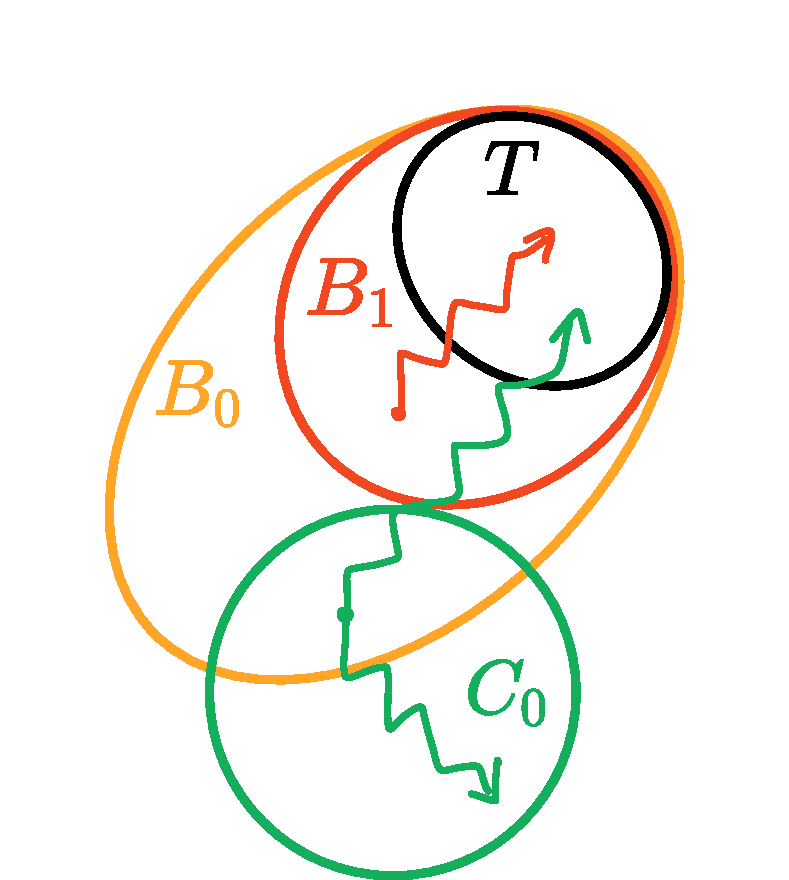
\includegraphics[width=0.5\linewidth]{figures/watr_illustration.pdf}
    \caption{Illustration showing the construction of weak attractors. In the area $B_0\setminus B_1$ player $i$ cannot enforce reaching $T$ without visiting $C_0$.}
    \label{fig:ill:watr}
\end{figure}

\begin{mytheorem}{Weak Attractors Compute AS-Reachability}{prop:asreach}\label{prop:asreach}
    Let $\mathcal{G} = (\set{0, 1}, S, A, \set{S_0, S_1}, \Delta, AP, \chi)$ be a two-player SMG and\\
    $\mathcal{P}=(S_0, S_1, S_N, E)$ be the corresponding RGN. It holds that:\[
        \watr_i(T, \mathcal{P})\cap S = \ASReach_i(T, \mathcal{G})\hspace{1.5cm}i\in\set{0, 1}
        \]
\end{mytheorem}
    

    
\begin{proof}
To prove theorem~\ref{prop:asreach}, we begin by showing a few helpful statements. First, observe that for all $k\in\N$:
\begin{align}
B_{k+1}\cap S\subseteq B_k\cap S \text{ and } C_{k+1}\cap S\supseteq C_k\cap S. \label{eq:mono_B_k_C_k}
\end{align}
We show this by induction over $k$: For $k=0$, it holds that $B_1\cap S = \Reach_i(T, \mathcal{G}\setminus C_0)$. Any strategy used by player $1$ to reach $T$ in the game $\mathcal{G}\setminus C_0$ also works in the larger game $\mathcal{G}$. Otherwise, there would need to be a state $s\in\mathcal{G}\setminus C_0$ belonging to player $1-i$, from which they can force the play out of $\mathcal{G}\setminus C_k$, but such a state would be in $\Reach_{1-i}(S\setminus B_0, \mathcal{G}\setminus T)=C_0\cap S$ and thus not in $\mathcal{G}\setminus C_0$. Therefore, it holds that $B_{1}\cap S\subseteq B_0\cap S$.

Furthermore, $\Reach_{1-i}(S\setminus B_1, \mathcal{G}\setminus T) = C_1\cap S\supseteq C_0\cap S = \Reach_{1-i}(S\setminus B_0, \mathcal{G}\setminus T)$, as $S\setminus B_1\supseteq S\setminus B_0$.

Now let equation~\ref{eq:mono_B_k_C_k} hold for a $k\in\N$. With the same reasoning as above, any strategy used by player $1$ to reach $T$ in the game $\mathcal{G}\setminus C_{k+1}$ also works in the larger game $\mathcal{G}\setminus C_{k}$. Thus $B_{k+1}\cap S = \Reach_i(T, \mathcal{G}\setminus C_k)\subseteq \Reach_i(T, \mathcal{G}\setminus C_{k-1})=B_{k}\cap S$.

Similarly to above, it also holds that: $\Reach_{1-i}(S\setminus B_{k+1}, \mathcal{G}\setminus T) = C_{k+1}\cap S\supseteq C_k\cap S = \Reach_{1-i}(S\setminus B_k, \mathcal{G}\setminus T)$, as $S\setminus B_{k+1}\supseteq S\setminus B_k$. Thus, equation~\ref{eq:mono_B_k_C_k} holds by induction.

Because of this, we can choose an $l\in\N$, such that $B_l\cap S = B_{l+1}\cap S$ and $C_l\cap S = C_{l+1}\cap S$ (such an $l$ exists because $S$ is finite). It holds by the definition of $\watr_i$ that
\begin{align}
\watr_i(T, \mathcal{P})\cap S&\stackrel{\ref{eq:mono_B_k_C_k}}{=}B_l\cap S\nonumber\\
&=\satr_i(T, \mathcal{P}\setminus C_l)\cap S\nonumber\\
&\stackrel{\ref{prop:reach}}{=}\Reach_i(T, \mathcal{G}\setminus C_l)\label{eq:satr_l}
\intertext{and}
C_l\cap S &= \satr_{1-i}(S\setminus B_l, \mathcal{P}\setminus T)\cap S\nonumber\\
&\stackrel{\ref{prop:reach}}{=} \Reach_{1-i}(S\setminus B_l, \mathcal{G}\setminus T)\nonumber\\
&= \Reach_{1-i}(S\setminus \watr_i(T, \mathcal{P}), \mathcal{G}\setminus T).\label{eq:C_l}
\end{align}

To show \say{$\subseteq$} of theorem~\ref{prop:asreach}, let $s\in\watr_i(T, \mathcal{P})$. By equation~\ref{eq:satr_l}, there is an $l\in\N$ such that $s\in\Reach_i(T, \mathcal{G}\setminus C_l)$. Let $\sigma_i^\ast$ be the corresponding strategy of player $i$ to reach $T$ in the game $\mathcal{G}\setminus C_l$, and let $\sigma_{1-i}$ be an arbitrary strategy for player $1-i$. It holds that $\Pr_s^{(\sigma_0^\ast, \sigma_1)}(\Reach(T)) > 0$. For the sake of contradiction, assume that for some $\sigma_i$, it holds that $\Pr_s^{(\sigma_0, \sigma_1)}(\Reach(T))< 1$. This means either there is a strategy $\sigma_{1-i}$, such that, with a positive probability, the play leaves $\watr_i(T, \mathcal{P})$ without visiting $T$ (case 1), or the play stays in $\watr_i(T, \mathcal{P})\setminus T$ indefinitely with a positive probability (case 2).

\begin{description}
    \item[Case 1:] It holds that $\forall\sigma_i\exists\sigma_{1-i}:\Pr_s^{(\sigma_0, \sigma_1)}(\Reach(S\setminus\watr_i(T, \mathcal{P}))\cap (S\setminus T)^\omega) > 0$. By determinacy (see theorem~\ref{theo:reach_det}) the player $1-i$ has a strategy $\sigma_{1-i}'$ such that $\forall\sigma_i: \Pr_s^{(\sigma_0, \sigma_1)}(\Reach(S\setminus\watr_i(T, \mathcal{P}))\cap (S\setminus T)^\omega) > 0$ and therefore $s\in C_l\cap S\stackrel{\ref{eq:C_l}}{=}\Reach_{1-i}(S\setminus \watr_i(T, \mathcal{P}), \mathcal{G}\setminus T)$, which is a contradiction to $s\in\Reach_i(T, \mathcal{G}\setminus C_l)$.
    

    \item[Case 2:] In this case, let $W\coloneqq\watr_i(T,\mathcal{P})\setminus T$ and let $P\coloneqq (WA)^\omega$ denote the set of paths that always stay in $W$. It holds that $\forall\sigma_i\exists\sigma_{1-i}: \Pr_s^{(\sigma_0, \sigma_1)}(P) > 0$.
    
    Observe that for any $s'\in W$ it cannot hold, that a state inside $W$ is visited twice with probability $1$:\[
    \forall\sigma_i\exists\sigma_{1-i}: \Pr_{s'}^{(\sigma_0, \sigma_1)}(s'A(WA)^\ast s'(SA)^\omega) = 1\] Otherwise a strategy $\sigma_{1-i}$ can be constructed for always staying in $W$ by repeatedly visiting $s'$, and by determinacy, this would mean that $s'\notin\Reach_i(T, \mathcal{G}\setminus C_l)$. Let $p_{s'}<1$ denote the minimal probability with \[
    \forall\sigma_i\exists\sigma_{1-i}: \Pr_{s'}^{(\sigma_0, \sigma_1)}(s'A(WA)^\ast s'(SA)^\omega) < p_{s'}\].
    
    As $W$ has finitely many states, every path inside $P$ has to include at least one state infinitely often. This means $P$ can be rewritten as: \begin{align*}
        P&=\bigcup_{s\in W}\bigcap_{n\in\N}(sA(WA)^\ast)^n(WA)^\omega\\
        \intertext{Using this, we can give an upper bound of $\Pr_s^{(\sigma_0, \sigma_1)}(P)$:\footnotemark}
        \Pr_s^{(\sigma_0, \sigma_1)}(P)&=\Pr_s^{(\sigma_0, \sigma_1)}\left(\bigcup_{s\in W}\bigcap_{n\in\N}(sA(WA)^\ast)^n(WA)^\omega\right)\\
        &\leq\sum_{s\in W}\Pr_s^{(\sigma_0, \sigma_1)}\left(\bigcap_{n\in\N}(sA(WA)^\ast)^n(WA)^\omega\right)\\
        \intertext{The probability of each set of paths $(sA(WA)^\ast)^n(WA)^\omega$ is bounded by $p_{s}^n$, as the probability revisiting $s$ once is bounded by $p_s$:}
        \Pr_s^{(\sigma_0, \sigma_1)}(P)&\leq\sum_{s\in W}p_s^n\quad\text{for all }n\in\N\\
        &=|W|\cdot p^n\quad\text{for all }n\in\N\\
        \intertext{Therefore, as $p<1$ and $|W|$ finite:}
        \Pr_s^{(\sigma_0, \sigma_1)}(P)&=0.
    \end{align*}
    This is a contradiction to $\forall\sigma_0\exists\sigma_1: \Pr_s^{(\sigma_0, \sigma_1)}(P) > 0$.
\end{description}
\footnotetext{Note that $P$ is measurable by $\Pr_s^{(\sigma_0, \sigma_1)}$ as it is a countable boolean combination of sets in the $\sigma$-algebra.}

As both cases lead to a contradiction, it must hold that $\Pr_s^{(\sigma_0^\ast, \sigma_1)}(\Reach(T)) = 1$ for any $\sigma_{1-i}$. And therefore $s\in\ASReach(T, \mathcal{G}\setminus C_l)$. Finally, note that the strategy $\sigma_0^\ast$ also works for the larger game $\mathcal{G}$. Otherwise, there would need to be a state $s\in\setminus C_l$ belonging to the player $1-i$, from which they can force the play out of $\mathcal{G}\setminus C_l$ before reaching $T$, but such a state would be in $\Reach_{1-i}(S\setminus \watr_i(T, \mathcal{P}), \mathcal{G}\setminus T)=C_l\cap S$ and thus not in $s\in\mathcal{G}\setminus C_l$. Thus, $s\in\ASReach(T, \mathcal{G})$.

To show \say{$\supseteq$} of theorem~\ref{prop:asreach}, let $s\notin S\cap\watr_i(T, \mathcal{P})$, this means $s\notin\Reach_i(T, \mathcal{G}\setminus C_l)$. Thus, in the game $\mathcal{G}\setminus C_l$, it holds that $\forall\sigma_i\exists\sigma_{1-i}\Pr(\Reach(T))<1$ and by determinacy player $1-i$ has a strategy $\sigma_{1-i}'$ for not reaching $T$ with a positive probability. We can differentiate between two cases:
\begin{description}
    \item[Case 1:] Player $i$ is not able to force the play out of $\mathcal{G}\setminus C_l$. In this case, $\sigma_{1-i}'$ is also a strategy for not reaching $T$ in the game $\mathcal{G}$.
    \item[Case 2:] Player $i$ is able to force the play out of $\mathcal{G}\setminus C_l$ to a state $s'\in C_l$ with a positive probability. Then player $1-i$ has a strategy to reach $S\setminus B_l$, as $s'\in\Reach_{1-i}(S\setminus B_l, \mathcal{G}\setminus T)$. For $s\in S\setminus B_l$, it holds that $s\notin\Reach_i(T, \mathcal{G}\setminus C_{l-1})$, which means in the game $\mathcal{G}\setminus C_{l-1}$ it holds that $\forall\sigma_i\exists\sigma_{1-i}\Pr(\Reach(T))<1$.
 Similarly to above, this means that player $1-i$ either has a strategy for not reaching $T$ in $\mathcal{G}$, or, if player $i$ forces the play to a state $s''\in C_{l-1}$, $s''\in\Reach_{1-i}(S\setminus B_{l-1}, \mathcal{G}\setminus T)$.
 \end{description}
 In this fashion, we can recursively construct a strategy for player $1-i$; in the last step, player $1-i$ can force the play out of $B_0=\satr_i(T, \mathcal{P})$ and as there are only finitely many steps, we end up with a strategy that has a positive probability of not reaching $T$ in the game $\mathcal{G}$.
 
Therefore, $s\notin\ASReach(T, \mathcal{G})$.
\end{proof}

\begin{mycorollary}{Memoryless Strategy for AS-Reachability}{lem:memless_watr}\label{lem:memless_watr}
There is a memoryless strategy for player $i$ to reach a target set $T$ with probability $1$.
\end{mycorollary}
\begin{proof}
The strategy constructed in the proof for theorem \ref{prop:asreach} is memoryless.
\end{proof}

\begin{figure}[t]
\centering
\begin{tikzpicture}[>=stealth, node distance=2.5cm, every node/.style={font=\small}]
    % Nodes
    \node[draw, minimum size=1cm, shape=rectangle] (S1) {$s_1$};
    \node[draw, minimum size=1cm, shape=circle, right=of S1] (S2) {$\textcolor{myred}{s_2}$};
    \node[draw, minimum size=1cm, shape=rectangle, right=of S2] (S3) {$\textcolor{myred}{s_3}$};
    \node[draw, minimum size=1cm, shape=circle, right=of S3] (S4) {$\textcolor{myblue}{s_4}$};

    % Self-loops
    \draw[->] (S1) edge[loop above]
        node[above, pos=0.5] {$(s_1, a)$} 
        coordinate[pos=0.5] (S1loop) (S1);
    \filldraw[black] (S1loop) circle (2pt);

    \draw[->] (S3) edge[loop above]
        node[above, pos=0.5] {$\textcolor{myred}{(s_3, a)}$} 
        coordinate[pos=0.5] (S3loop) (S3);
    \filldraw[black] (S3loop) circle (2pt);

    \draw[->] (S4) edge[loop above]
        node[above, pos=0.5] {$\textcolor{myblue}{(s_4, a)}$} 
        coordinate[pos=0.5] (S4loop) (S4);
    \filldraw[black] (S4loop) circle (2pt);

    % Transitions and splits
    \draw[-] (S1) -- node[below] {} ($(S1)!0.5!(S2)$);
    \filldraw[black] ($(S1)!0.5!(S2)$) circle (2pt) 
        node[label={90:$\textcolor{myred}{(s_1, b)}$}] {}; % Labeled split point
    \draw[->] ($(S1)!0.5!(S2)$) -- (S2);
    \draw[->] ($(S1)!0.5!(S2)$) .. controls +(0,-1) and +(0,-1) .. node[below] {} (S1);

    \draw[-] (S2) -- node[below] {} ($(S2)!0.5!(S3)$);
    \filldraw[black] ($(S2)!0.5!(S3)$) circle (2pt) 
        node[label={90:$\textcolor{myred}{(s_2, b)}$}] {};
    \draw[->] ($(S2)!0.5!(S3)$) -- (S3);
    \draw[->] ($(S2)!0.5!(S3)$) .. controls +(0,-2) and +(0,-2) .. node[below] {} (S1);

    \draw[-] (S3) -- node[below] {} ($(S3)!0.5!(S4)$);
    \filldraw[black] ($(S3)!0.5!(S4)$) circle (2pt) 
        node[label={90:$\textcolor{myblue}{\textcolor{myblue}{(s_3, b)}}$}] {};
    \draw[->] ($(S3)!0.5!(S4)$) -- (S4);
    \draw[->] ($(S3)!0.5!(S4)$) .. controls +(0,-3) and +(0,-3) .. node[below] {} (S1);

    % No transition from S4 to S1
\end{tikzpicture}

\caption{An example of a RGN that serves to illustrate the calculation of the weak attractor of the target set $\set{s_1}$ for the square player. In each iteration $C_k$ includes more states, until only $s_1$ and $(s_1, a)$ remain in the weak attractor.}
\label{fig:example_game_02_watr}
\end{figure}
\begin{myexample}{Weak Attractors}{ex:watr}
Let $\mathcal{P}=(\set{s_1, s_3}, \set{s_2, s_4}, \set{(s_1, a), (s_1, b), (s_2, b), (s_3, a), (s_3, b), (s_4, a)}, E)$ be the RGN shown in figure~\ref{fig:example_game_02_watr}, with the square nodes representing player $0$ and the circular nodes representing player $1$. The weak attractor of $T\defeq\set{s_1}$ for player $0$, $\watr_0(\set{s_1}, \mathcal{P})$, can be computed as follows:
\begin{align*}
    B_0 &= \set{s_1, s_2, s_3, (s_1, a), (s_1, b), (s_2, b), (s_3, a), (s_3, b)}\\
    C_0 &= \set{\textcolor{myblue}{s_4}, \textcolor{myblue}{(s_3, b)}, \textcolor{myblue}{(s_4, a)}}\\
    B_1 &= \set{s_1, s_2, (s_1, a), (s_1, b), (s_2, b)}\\
    C_1 &= \set{\textcolor{myred}{s_2}, \textcolor{myred}{s_3}, s_4, \textcolor{myred}{(s_1, b)}, \textcolor{myred}{(s_2, b)}, \textcolor{myred}{(s_3, a)}, (s_3, b), (s_4, a)}\\
    B_2 &= \set{s_1, (s_1, a)}\\
    C_k &= C_1\quad\text{ for }k\geq 1\\
    B_k &= B_2\quad\text{ for }k\geq 2\\
\watr_0(\set{s_1}, \mathcal{P})&=\set{s_1, (s_1, a)}
\end{align*}
Note that at first $s_3$ is not included in $C_0$ as player $0$ can prevent player $1$ from reaching $S\setminus B_0$ by always taking the self loop. But it is not included in $B_1$ as player $0$ is no longer allowed to utilize the nature state $(s_3, b)$. Therefore, it is included in $C_1$, as well as the states from which player $1$ can enforce reaching $s_3$.
\end{myexample}

\section{Algorithm}
\label{sec:algorithm}
\begin{algorithm}[t!]
    \caption{Computation of Strong Attractors}\label{alg:satr}
    \begin{algorithmic}[1]
        \Procedure{StrongAttractors}{$S_0, S_1, A, \Delta, i, T, S_\text{allowed}, \Delta_\text{allowed}$}
            \State $\satr\gets  T$
            \State $\Delta_{\satr} \gets\emptyset$
            \State $B\gets T$

            \While{$B\neq\emptyset$}
                \State $P\gets\Pred_\Delta(B)\setminus\satr$\label{alg:satr:pred}
                \State $B\gets\emptyset$
                \ForAll{$s\in P, a\in A$ with $\Delta(s, a)\neq\bot$}\label{alg:satr:bdelta}
                        \If{$\Succ_\Delta((s, a))\cap\satr\neq\emptyset$ \textbf{and} $(s, a)\in\Delta_\text{allowed}$}
                            \State $\Delta_{\satr}\gets \Delta_{\satr}\cup\set{(s, a)}$
                        \EndIf
                \EndFor\label{alg:satr:edelta}
                \State $P\gets P\cap S_\text{allowed}$\label{alg:satr:allowed}
                \ForAll{$s\in P$}\label{alg:satr:bcheck}
                    \If{$s\in S_i$}
                        \If{there exists a $a\in A(s)$ with $(s, a)\in\Delta_{\satr}$}
                            \State $B\gets\set{s}$
                        \EndIf
                    \Else
                        \If{for all $a\in A(s)$ it holds that $(s, a)\in\Delta_{\satr}$}
                            \State $B\gets\set{s}$
                        \EndIf
                    \EndIf
                \EndFor\label{alg:satr:echeck}
                \State $\satr\gets\satr\cup B$
            \EndWhile
            \State \textbf{return} $\satr, \Delta_{\satr}$
        \EndProcedure
    \end{algorithmic}
\end{algorithm}
\begin{algorithm}[t!]
    \caption{Computation of Weak Attractors}\label{alg:watr}
    \begin{algorithmic}[1]
        \Procedure{WeakAttractors}{$S_0, S_1, A, \Delta, i, T, S_\text{allowed}$}
            \State $B\gets T$
            \State $\Delta_\text{allowed}\gets (S_0\cup S_1)\times A$
            \State $B_\text{next}, \Delta_{B, \text{next}}\gets $ \Call{StrongAttractors}{$S_0, S_1, A,\Delta, i, T, S_\text{allowed}, \Delta_\text{allowed}$}
            \While{$B\neq B_\text{next}$}
                \State $B\gets B_\text{next}$
                \State $T_C\gets(S_0\cup S_1)\setminus B$
                \State $S_{\text{allowed}, C}\gets S_\text{allowed}\setminus T$
                \State $C, \Delta_C\gets$ \Call{StrongAttractors}{$S_0, S_1, A,\Delta, 1-i, T_C, S_{\text{allowed}, C}, \Delta_\text{allowed}$}
                \State $S_{\text{allowed}, B}\gets S_\text{allowed}\setminus C$
                \State $\Delta_{\text{allowed}, B}\gets \Delta_\text{allowed}\setminus \Delta_C$
                \State $B_\text{next}, \Delta_{B, \text{next}}\gets $ \Call{StrongAttractors}{$S_0, S_1, A,\Delta, i, T, S_{\text{allowed}, B}, \Delta_{\text{allowed}, B}$}
            \EndWhile
        \EndProcedure
        \State \textbf{return} $B$
    \end{algorithmic}
\end{algorithm}

Algorithm~\ref{alg:satr} describes the procedure for computing strong attractors. The input consists of a two-player SMG $\mathcal{G} = (\set{0, 1}, S, A, \set{S_0, S_1}, \Delta, AP, \chi)$. We assume a sparse matrix representation of the transition relation $\Delta$, which enables efficient lookup of the predecessor states of state $s$
($\Pred_\Delta(s)\defeq \{s' \in S \mid \exists a \in A(s) \text{ with } \Delta(s', a)(s) > 0\}$), the available actions of the state ($A(s)$), and the successor states for a given action $a \in A(s)$ ($\Succ_\Delta((s, a)) \defeq \{s' \in S \mid \Delta(s, a)(s') > 0\}$).

The procedure \texttt{StrongAttractors}$(S_0, S_1, A, \Delta, i, T, S_\text{allowed}, \Delta_\text{allowed})$ computes the strong attractor $\satr_i(T, \mathcal{P})$ where $\mathcal{P} = (S_0 \cap S_\text{allowed}, S_1 \cap S_\text{allowed}, \Delta_\text{allowed}, E)$. This is done in layers, with each iteration computing a new set of states $B \subseteq S$ and updating the set of nature states $\Delta_{\satr}$.

In the first step, we initialize the strong attractor set $\satr \gets T$ and the set of nature states $\Delta_{\satr} \gets \emptyset$. In each iteration, we first compute the predecessors $P$ of the previous layer $B$ (line~\ref{alg:satr:pred}), excluding those already in $\satr$. 

We update the set of nature states in the strong attractor by considering the outgoing edges of $P$ (lines~\ref{alg:satr:bdelta} to~\ref{alg:satr:edelta}). After updating $\Delta_{\satr}$, we filter $P$ to only include the allowed states (line~\ref{alg:satr:allowed}). This step is performed after updating $\Delta_{\satr}$ because we would otherwise miss allowed nature states that are successors of disallowed states.

For each state $s \in P$, we check if it can be added to the strong attractor. If $s$ belongs to player $i$, we check if there is a following nature state in $\Delta_{\satr}$. This check is necessary because the connecting nature state might be disallowed, even if $s$ is a predecessor of $\satr$. If $s$ belongs to the other player, all following nature states must be in $\Delta_{\satr}$ for $s$ to be added to the attractor (lines~\ref{alg:satr:bcheck} to~\ref{alg:satr:echeck}).

\begin{figure}[t]
\centering
\begin{tikzpicture}[>=stealth, node distance=1.8cm, every node/.style={font=\small}]
    % Nodes for s chain
    \node[draw, minimum size=1cm, shape=rectangle] (S1) {$s_1$};
    \node[draw, minimum size=1cm, shape=rectangle, right=of S1] (S2) {$s_2$};
    \node[draw, minimum size=1cm, shape=rectangle, draw=none, right=of S2] (dots) {\dots};
    \node[draw, minimum size=1cm, shape=rectangle, right=of dots] (Snm1) {$s_{n-1}$};
    \node[draw, minimum size=1cm, shape=rectangle, right=of Snm1] (Sn) {$s_n$};

    % Nodes for t chain
    \node[draw, minimum size=1cm, shape=rectangle, above=1.8cm of S1] (T1) {$t_1$};
    \node[draw, minimum size=1cm, shape=rectangle, right=of T1] (T2) {$t_2$};
    \node[draw, minimum size=1cm, shape=rectangle, draw=none, right=of T2] (dotsT) {\dots};
    \node[draw, minimum size=1cm, shape=rectangle, right=of dotsT] (Tnm1) {$t_{n-1}$};
    \node[draw, minimum size=1cm, shape=rectangle, right=of Tnm1] (Tn) {$t_n$};

    % Self-loops for s chain

    \draw[->] (S2) edge[loop above]
        node[above, pos=0.5] {$(s_2, a)$} 
        coordinate[pos=0.5] (S2loop) (S3);
    \filldraw[black] (S2loop) circle (2pt);
    
    \draw[->] (Snm1) edge[loop above]
        node[above, pos=0.5] {$(s_{n-1}, a)$} 
        coordinate[pos=0.5] (Snm1loop) (S3);
    \filldraw[black] (Snm1loop) circle (2pt);
    
    \draw[->] (Sn) edge[loop above]
        node[above, pos=0.5] {$(s_{n}, a)$} 
        coordinate[pos=0.5] (Snloop) (S3);
    \filldraw[black] (Snloop) circle (2pt);

    
    % t_n selfloop
    \draw[->] (Tn) edge[loop above]
        node[above, pos=0.5] {$(t_{n}, a)$} 
        coordinate[pos=0.5] (Tnloop) (S3);
    \filldraw[black] (Tnloop) circle (2pt);

    % Transitions within s chain
    \draw[-] (S1) -- node[below] {} ($(S1)!0.5!(S2)$);
    \filldraw[black] ($(S1)!0.5!(S2)$) circle (2pt) node[label={90:$(s_1, b)$}] {};
    \draw[->] ($(S1)!0.5!(S2)$) -- (S2);
    \draw[->] ($(S1)!0.5!(S2)$) .. controls +(0,-1) and +(0,-1) .. node[below] {} (S1);

    \draw[-] (S2) -- node[below] {} ($(S2)!0.5!(dots)$);
    \filldraw[black] ($(S2)!0.5!(dots)$) circle (2pt) node[label={90:$(s_2, b)$}] {};
    \draw[->] ($(S2)!0.5!(dots)$) -- (dots);
    \draw[->] ($(S2)!0.5!(dots)$) .. controls +(0,-1.5) and +(0,-1.5) .. node[below] {} (S1);

    \draw[-] (dots) -- node[below] {} ($(dots)!0.5!(Snm1)$);
    \filldraw[black] ($(dots)!0.5!(Snm1)$) circle (2pt) node[label={90:$(s_{n-2}, b)$}] {};
    \draw[->] ($(dots)!0.5!(Snm1)$) -- (Snm1);
    \draw[->] ($(dots)!0.5!(Snm1)$) .. controls +(0,-2) and +(0,-2) .. node[below] {} (S1);

    \draw[-] (Snm1) -- node[below] {} ($(Snm1)!0.5!(Sn)$);
    \filldraw[black] ($(Snm1)!0.5!(Sn)$) circle (2pt) node[label={90:$(s_{n-1}, b)$}] {};
    \draw[->] ($(Snm1)!0.5!(Sn)$) -- (Sn);
    \draw[->] ($(Snm1)!0.5!(Sn)$) .. controls +(0,-3) and +(0,-3) .. node[below] {} (S1);

    % Transitions from s chain to t chain
    \draw[-] (S1) -- node[below] {} ($(S1)!0.5!(T1)$);
    \filldraw[black] ($(S1)!0.5!(T1)$) circle (2pt) node[label={180:$(t_1, a)$}] {};
    \draw[->] ($(S1)!0.5!(T1)$) -- (T1);

    \draw[-] (T1) -- node[below] {} ($(T1)!0.5!(T2)$);
    \filldraw[black] ($(T1)!0.5!(T2)$) circle (2pt) node[label={90:$(t_2, a)$}] {};
    \draw[->] ($(T1)!0.5!(T2)$) -- (T2);

    \draw[-] (T2) -- node[below] {} ($(T2)!0.5!(dotsT)$);
    \filldraw[black] ($(T2)!0.5!(dotsT)$) circle (2pt) node[label={90:$(t_{n-2}, a)$}] {};
    \draw[->] ($(T2)!0.5!(dotsT)$) -- (dotsT);

    \draw[-] (dotsT) -- node[below] {} ($(dotsT)!0.5!(Tnm1)$);
    \filldraw[black] ($(dotsT)!0.5!(Tnm1)$) circle (2pt) node[label={90:$(t_{n-1}, a)$}] {};
    \draw[->] ($(dotsT)!0.5!(Tnm1)$) -- (Tnm1);

    \draw[-] (Tnm1) -- node[below] {} ($(Tnm1)!0.5!(Tn)$);
    \filldraw[black] ($(Tnm1)!0.5!(Tn)$) circle (2pt) node[label={90:$(t_n, a)$}] {};
    \draw[->] ($(Tnm1)!0.5!(Tn)$) -- (Tn);

\end{tikzpicture}
\caption{A RNG that shows the worst-case complexity of the procedure for weak attractors. In the calculation of the weak attractor of $\set{t_0}$ for the square player. In the $k$-iteration, $s_{n-k}$ is the only non-nature state added to $C_k$. Therefore $O(n)$ iterations are needed. Whereas the computation of $B_k$ requires traversing the $n$ states of the upper chain ($t_1$, ..., $t_n$), taking $O(|\Delta|)$ steps. }
\label{fig:example_worst_case}
\end{figure}

\begin{mytheorem}{Computational Complexity of Positive Reachability}{theo:satr_runtime}
Let $\mathcal{G}$ be a two-player SMG and $T$ a set of target states. It holds that:

Calculating the set $\Reach_i(T, \mathcal{G})$ for a player $i\in\set{0,1}$ using the \texttt{StrongAttractors} procedure takes $\Theta(|\Delta|)$ computational steps in the worst case.
\end{mytheorem}
\begin{proof}
The procedure \texttt{StrongAttractors} calculates $\Reach_i(T, \mathcal{G})$. Every state of $\mathcal{G}$ is added at most once to the working set $B$. In each iteration, we iterate over all outgoing transitions of the states in $B$. Therefore, we consider each transition at most once and need at most $O(|\Delta|)$ computational steps.

On the other hand, figure~\ref{fig:example_worst_case} shows an RNG for which the \texttt{StrongAttractors} procedure explores every transition except $(s_n, a)$ when calculating  $\Reach_0(\set{t_n}, \mathcal{G})$. Thus taking $|\Delta|$ steps.
\end{proof}

By processing the states in layers, we ensure that the successors of each state are considered only once, leading to a runtime of $O(|\Delta|)$.

Finally, the procedure returns the of set states $\satr$ and nature states $\Delta_{\satr}$ of the strong attractor.

Algorithm~\ref{alg:watr} describes the procedure for computing weak attractors. It closely mirrors the definition of weak attractors in section \ref{sec:watr}. It alternately calls the \texttt{StrongAttractors} procedure for both players, until a fixed point is reached.

\begin{mytheorem}{Computational Complexity of Almost Sure Reachability}{theo:watr_runtime}
Let $\mathcal{G}$ be a two-player SMG and $T$ a set of target states. It holds that:

Calculating the set $\ASReach_i(T, \mathcal{G})$ for a player $i\in\set{0,1}$ using the \texttt{WeakAttractors} procedure takes $\Theta(|S|\cdot|\Delta|)$ computational steps in the worst case.
\end{mytheorem}
\begin{proof}
In every iteration at least one non-nature state is removed $B$ and the \texttt{StrongAttractors} procedure is called a constant amount of times. Therefore the algorithm takes at most $|S|$ iterations and $O(|S|\cdot\Delta)$ steps.

On the other hand, figure~\ref{fig:example_worst_case} shows an RNG for which in the $k$-th iteration the state $s_{n-k}$ is included in $B_k$, and then newly added to $C_k$ and consequently not included in the set $B_{k+1}$. Therefore, at least $\frac{|S|}{2}-2\in O(|S|)$ iterations are needed. In each iteration the calculation of $B_k$ involves traversing the upper chain of states ($t_1, \dots, t_n$), taking at least $\frac{|\Delta|}{3}\in\Omega(|\Delta|)$ steps. Therefore, in the worst case, the algorithm takes $\Omega(|\Delta|)$ steps.
\end{proof}
\chapter{Experimental Evaluation}
\label{chap:eval}

\section{Implementation in Storm}
\label{sec:storm_implementation}

Storm is a probabilistic model checker that supports a variety of models, including discrete- and continuous-time Markov chains, Markov decision processes, and modeling languages such as PRISM and JANI. It is implemented in C++ and is designed to be extensible. Storm performed best on the QComp 2019 benchmark set \cite{hensel_probabilistic_2020, hahn_2019_2019}, but does not support SMG model checking.

\subsection*{Implementation Details\footnote{Our source code is publicly available on GitHub: \url{https://github.com/weiss-i-net/storm}}}
The modular design of Storm facilitated the integration of the stochastic game algorithms without requiring extensive modifications to the existing codebase. However, the large size of the codebase (approximately 170,000 lines of code) posed challenges in understanding and working with the architecture.

The implementation supports properties of the form:
\[
\langle\langle C \rangle\rangle\;\mathsf{P}\vartriangle p\; [\phi_1 \, \until \, \phi_2],
\]
where $C$ is a coalition of players, $\vartriangle \in \{<, \leq, =, \geq, >\}$, $p \in \set{0, 1}$, and $\phi_1, \phi_2$ are subformulas. All states belonging to the specified coalition are assigned to Player $0$, while the remaining states are assigned to Player $1$.

Storm recursively calculates the sets of states satisfying $\phi_1$ and $\phi_2$, referred to as $\Phi_1$ and $\Phi_2$, respectively. Using these sets, the implementation computes $\Reach_0(\Phi_2, \mathcal{G})$, applying a modified version of the strong attractors routine that restricts Player $0$ to states within $\Phi_1$.

\begin{lstfloat}
\begin{lstlisting}[
    language=C++,
    caption={A code snippet illustrating the use of C++20's ranges. Instead of using nested for-loops, a range of elements is passed through multiple transformations (so-called range adaptors).},
    label={lst:ranges}
]
auto transitionIndexView = predecessorStates
    | std::views::transform([&](auto const index) {
        return transitionMatrix.getRowGroupIndices(index);
    }) 
    | std::views::join
    | std::views::filter([&](auto const index) {
        return allowedTransitions.get(index);
    })
    | std::views::filter(transitionLeadsToAttractors);

for (auto const index : transitionIndexView) {
    transitionsLeadingToAttractors.set(index);
}
\end{lstlisting}

\end{lstfloat}

As Storm recently adopted C++20, we were able to use modern language features, such as ranges and range adaptors, to implement the code in a functional style. Listing~\ref{lst:ranges} illustrates this. In this snippet, we compute the set of transitions leading into the set of strong attractors from the previous iteration. Instead of a nested for-loop, we start with a range of states, transform it into a range of ranges of outgoing transitions, flatten it into a single range of transitions, and filter out the transitions that are not allowed or do not lead to the attractor set. Note that the resulting \texttt{transitionIndexView} variable is lazily evaluated.

\section{PRISM-games}
\label{sec:prism}

PRISM-games is the first comprehensive tool for model checking stochastic games \cite{hutchison_prism-games_2013}. Built on the PRISM model checker \cite{kwiatkowska_prism_2011}, it introduces the rPATL logic for expressing properties of SMGs, which is also used by Storm. The tool is implemented in Java.

PRISM-games employs a nested fixpoint computation for AS-reachability in SMGs, which is similar to our algorithm. However, a key distinction lies in the computation of positive reachability (strong attractors). PRISM-games iterates over all states repeatedly, checking whether each state’s successors belong to the working set and meet the inclusion criteria. In contrast, our approach processes only the predecessors of each state in the working set, working backwards through layers.

A notable feature of PRISM-games is its support for calculations on symbolically represented SMGs. Instead of explicitly storing every state and its successors in a transition matrix, the tool uses multi-terminal binary decision diagrams (MTBDDs) to represent states and transitions compactly.

Both tools provide multiple \textit{engines} that can be selected during execution. For our evaluation, we focus on the \textit{explicit} and \textit{symbolic} engines (denoted as "dd" in diagrams), which correspond to the explicit and symbolic storage of the transition system, respectively. Our algorithm for AS-reachability in SMGs is only supported by the explicit engine, whereas PRISM-games supports both explicit and symbolic engines. Additionally, both tools allow the use of these engines for MDPs.


\section{Research Questions}
\label{sec:rqs}
To guide the experimental evaluation, we aim to explore the following research questions:
\begin{itemize}
    \item[\textbf{RQ1}:] How does the performance of our algorithm compare to the existing implementation in PRISM-games?
    \item[\textbf{RQ2}:] How much performance gain is achieved by performing the computations symbolically?
    \item[\textbf{RQ3}:] How does the performance of our algorithm, when run on MDPs, compare to existing implementations for MDPs in PRISM-games and Storm?
    \item[\textbf{RQ4}:] How does real-world performance compare to the worst-case performance?
\end{itemize}


\section{Test Cases}
\label{sec:test_cases}

To investigate the research questions outlined earlier, we consider the following test cases. Each case will be evaluated using the explicit engine for SMGs in Storm (our algorithm) and the explicit and symbolic engines for SMGs in PRISM-games. For MDPs, both Storm and PRISM-games offer explicit and symbolic engines, which will also be included in the evaluation.

\begin{enumerate}
    \item\label{test:swc} \textbf{Synthetic SMG with Theoretical Worst-Case Complexity (SWC):} 
    We use a synthetic stochastic multiplayer game (SMG) that theoretically exhibits an \(O(n \cdot m)\) run time complexity, as illustrated in Figure~\ref{fig:example_worst_case}. This test case is designed to examine the worst-case run time of our algorithm. As this SMG also represents an MDP (since it has only one player), we will evaluate its performance using the explicit and symbolic MDP engines in both Storm and PRISM-games.

    \item\label{test:inv} \textbf{Investor in a Futures Market (INV):} 
    This example models the expected wealth of an investor in a futures market, adapted from \cite{mciver_results_2003}. At discrete time steps (months), the investor can nondeterministically decide whether to reserve a stock for the next month. A month later, the stock is delivered, and the investor decides whether to sell it or not. The price of the stock follows a probabilistic distribution. This real-world scenario is chosen to evaluate practical performance. We will focus on reachability properties, verifying from which states the investor can almost surely reach the set of states where profit has been made. This test case will be evaluated using the explicit and symbolic engines for SMGs in PRISM-games and the explicit engine for SMGs in Storm. The model is dependant on two parameters the initial value \texttt{vinit} and the maximum value \texttt{vmax}. We set \texttt{vmax} to values between $2$ and $40$ and \texttt{vinit} to $\frac{\texttt{vmax}}{2}$, resulting in transition systems with between $1144$ and $6542393$ states.
\end{enumerate}

\subsection{Test Setup}
\label{subsec:test_setup}

All experiments were conducted on a laptop with the following specifications:

\begin{itemize}
    \item \textbf{Processor:} Intel Core i7-8650U
    \item \textbf{Memory:} 8 GB of RAM
    \item \textbf{Operating System:} Debian 12 running under Windows Subsystem for Linux (WSL) on Windows 11 (version H23H2).
\end{itemize}

The default configuration of WSL was adjusted to utilize the full 8 GB of RAM available on the system. For the experiments, the following software versions were used:

\begin{itemize}
    \item \textbf{Storm:} Version 1.9.0, which served as the basis for our implementation.
    \item \textbf{PRISM-games:} Version 3.2.1.
\end{itemize}

Each test case was executed until completion or until the process ran out of memory. Run time measurements were taken by parsing the reported run times for each stage of model checking from the output of the programs. This allowed us to isolate the time taken for calculating qualitative reachability, disregarding other steps such as model building and quantitative model checking performed by the programs. However, this approach has the drawback of limiting the resolution of the measurements to \(0.001\) seconds

\section{Results}
\label{sec:results}

\begin{figure}[t]
\centering
\begin{tikzpicture}
    \begin{loglogaxis}[
        axis equal,
        width=10cm,
        height=10cm,
        xmin=0.0005, xmax=160,
        ymin=0.0005, ymax=160,
        xlabel={Storm (s)},
        ylabel={PRISM-games (s)},
        legend pos=north west
    ]
    \addplot[only marks, mark=*, mark options={myorange}] table[x=storm_reachability, y=prism_reachability, col sep=comma] {figures/data/bad_runtime_example.csv};
    \addlegendentry{SWC}
    \addplot[only marks, mark=square*, mark options={mypink}] table[x=storm_reachability, y=prism_symbolic_reachability, col sep=comma] {figures/data/bad_runtime_example.csv};
    \addlegendentry{SWC (dd)}
    \addplot[only marks, mark=triangle*, mark options={myred}] table[x=storm_reachability, y=prism_reachability, col sep=comma] {figures/data/investor.csv};
    \addlegendentry{INV}
    \addplot[only marks, mark=diamond*, mark options={myblue}] table[x=storm_reachability, y=prism_symbolic_reachability, col sep=comma] {figures/data/investor.csv};
    \addlegendentry{INV (dd)}
    
    \addplot[domain=0.0005:160, samples=100, dashed] {x / 25}
    node[pos=0.32, anchor=160] {\tiny $\frac{1}{25}\times$};
    \addplot[domain=0.0005:160, samples=100, dashed] {0.2 * x}
    node[pos=0.23, anchor=160] {\tiny $\frac{1}{5}\times$};
    \addplot[domain=0.0005:160, samples=100, dashed] {x}
    node[pos=0.14, anchor=160] {\tiny $1\times$};
    \addplot[domain=0.0005:160, samples=100, dashed] {5 * x}
    node[pos=0.05, anchor=160] {\tiny $5\times$};
    \addplot[domain=0.0005:160, samples=100, dashed] {25 * x}
    node[pos=0.05, anchor=160] {\tiny $25\times$};
    \addplot[domain=0.0005:160, samples=100, dashed] {125 * x}
    node[pos=0.05, anchor=160] {\tiny $125\times$};
    \end{loglogaxis}
\end{tikzpicture}
\caption{Scatter plot of the run time for computing almost-sure reachability with our implementation in Storm compared to the run time of PRISM-games on various test cases. For PRISM-games both the explicit and the symbolic (dd) engines where used.}
\label{fig:plot_scatter}
\end{figure}

\subsection{Test Case \ref{test:swc}}
\pgfplotsset{compat=1.18}



\begin{figure}[t]
\centering
\begin{tikzpicture}
    \begin{loglogaxis}[
        xlabel={Number of States},
        ylabel={Time (s)},
        width=10cm,
        legend pos=north west,
    ]
    \addplot[myblue, mark=triangle*] table[x=number_of_states, y=storm_reachability, col sep=comma] {figures/data/bad_runtime_example.csv};
    \addlegendentry{Storm}

    \addplot[mygreen, mark=square*] table[x=number_of_states, y=prism_reachability, col sep=comma] {figures/data/bad_runtime_example.csv};
    \addlegendentry{PRISM-games}

    \addplot[mypink, mark=pentagon*] table[x=number_of_states, y=prism_symbolic_reachability, col sep=comma] {figures/data/bad_runtime_example.csv};
    \addlegendentry{PRISM-games (dd)}
    \end{loglogaxis}
\end{tikzpicture}
\caption{Run time comparison of Storm, PRISM-games (explicit), and PRISM-games (symbolic/dd) for almost-sure reachability checking on Test Case \ref{test:swc} (SWC)}
\label{fig:plot_swc}
\end{figure}




Figure \ref{fig:plot_swc} shows the performance of our implementation compared to PRISM-games on Test Case \ref{test:swc}. Our implementation significantly outperforms the explicit engine of PRISM-games across all tested transition system sizes. The parallel lines for larger numbers of states in the log-log plot indicate similar asymptotic behavior between the two implementations.

Figure \ref{fig:plot_scatter} highlights that our implementation is at least five times faster than the PRISM-games explicit engine for all tested system sizes. For smaller transition systems, the performance advantage increases to up to 50 times or more. However, we cannot confirm exact numbers for these cases, as Storm consistently reported the minimum runtime of $0.001$ seconds. This suggests that PRISM-games has a large constant runtime overhead compared to Storm. In contrast, the straight line for Storm indicates performance closely matching the expected asymptotic behavior with no measurable constant overhead.

Storm also outperforms PRISM-games' symbolic engine up to medium-sized transition systems (around 500 states). This behavior aligns with expectations, as symbolic representations typically excel with larger transition systems. For the largest tested systems, PRISM-games' symbolic engine is roughly five times faster than Storm. Interestingly, even for smaller transition systems, the symbolic engine of PRISM-games outperforms its explicit engine. This result deviates from the common expectation that simpler data structures (explicit representation) perform better on smaller test cases. This discrepancy can be attributed to PRISM-games' explicit engine being implemented in Java, whereas the symbolic operations on the MTBDD are implemented in C.


\begin{figure}[t]
\centering
\begin{tikzpicture}
    \begin{loglogaxis}[
        xlabel={Number of States},
        ylabel={Time (s)},
        width=10cm,
        legend pos=north west,
    ]
    \addplot[myblue, mark=triangle*] table[x=number_of_states, y=storm_model_building, col sep=comma] {figures/data/bad_runtime_example.csv};
    \addlegendentry{Storm}

    \addplot[mygreen, mark=square*] table[x=number_of_states, y=prism_model_building, col sep=comma] {figures/data/bad_runtime_example.csv};
    \addlegendentry{PRISM-games}

    \addplot[mypink, mark=pentagon*] table[x=number_of_states, y=prism_symbolic_model_building, col sep=comma] {figures/data/bad_runtime_example.csv};
    \addlegendentry{PRISM-games (dd)}
    \end{loglogaxis}
\end{tikzpicture}
\caption{Model building time comparison of Storm, PRISM-games (explicit), and PRISM (symbolic/dd) for Test Case \ref{test:swc} (SWC)}
\label{fig:plot_swc_build}
\end{figure}

Figure \ref{fig:plot_swc_build} shows the model building times for the test case. The symbolic engine exhibits significantly higher model building times compared to the explicit engine. This is because the model is provided explicitly; in such cases, the symbolic representation incurs additional overhead during model building. Faster model checking times can be achieved with the symbolic engine, but at the cost of longer model building times.

\subsection{Test Case \ref{test:inv}}

\pgfplotsset{compat=1.18}


\begin{figure}[t]
\centering
\begin{tikzpicture}
    \begin{loglogaxis}[
        xlabel={Number of States},
        ylabel={Time (s)},
        width=10cm,
        legend pos=north west,
    ]
    \addplot[myblue, mark=triangle*] table[x=number_of_states, y=storm_reachability, col sep=comma] {figures/data/investor.csv};
    \addlegendentry{Storm}

    \addplot[mygreen, mark=square*] table[x=number_of_states, y=prism_reachability, col sep=comma] {figures/data/investor.csv};
    \addlegendentry{PRISM-games}

    \addplot[mypink, mark=pentagon*] table[x=number_of_states, y=prism_symbolic_reachability, col sep=comma] {figures/data/investor.csv};
    \addlegendentry{PRISM-games (dd)}
    \end{loglogaxis}
\end{tikzpicture}
\caption{Run time comparison of Storm, PRISM-games (explicit), and PRISM-games (symbolic/dd) for almost-sure reachability checking on Test Case \ref{test:inv} (INV)}
\label{fig:plot_inv}
\end{figure}




Figure \ref{fig:plot_inv} shows the run times for the second test case. In this real-world example, the performance gap between Storm and PRISM-games increases significantly, with Storm outperforming PRISM-games by roughly 25 times (see Figure \ref{fig:plot_scatter}). Storm even outperforms PRISM-games' symbolic engine across all completed tests.

It is important to note that Storm did not finish for the largest input size, and the explicit engine of PRISM-games did not finish for the two largest input sizes, as both ran out of memory. As observed in Test Case \ref{test:swc}, constant overhead in PRISM-games is evident in this scenario as well. Parallel lines in the log-log plot for the explicit engines of PRISM-games and Storm again suggest similar asymptotic behavior.


\begin{figure}[t]
\centering
\begin{tikzpicture}
    \begin{loglogaxis}[
        xlabel={Number of States},
        ylabel={Time (s)},
        width=10cm,
        legend pos=north west,
    ]
    \addplot[myblue, mark=triangle*] table[x=number_of_states, y=storm_model_building, col sep=comma] {figures/data/investor.csv};
    \addlegendentry{Storm}

    \addplot[mygreen, mark=square*] table[x=number_of_states, y=prism_model_building, col sep=comma] {figures/data/investor.csv};
    \addlegendentry{PRISM-games}

    \addplot[mypink, mark=pentagon*] table[x=number_of_states, y=prism_symbolic_model_building, col sep=comma] {figures/data/investor.csv};
    \addlegendentry{PRISM-games (dd)}
    \end{loglogaxis}
\end{tikzpicture}
\caption{Model building time comparison of Storm, PRISM-games (explicit), and PRISM (symbolic/dd) for Test Case \ref{test:inv} (INV)}
\label{fig:plot_inv_build}
\end{figure}

Figure \ref{fig:plot_inv_build} shows the model building times for this test case. Unlike in the previous test case, the symbolic engine of PRISM-games demonstrates faster model building times for all but the smallest test cases.

\subsection{Test Case \ref{test:swc} as MDP}

In this section, we analyze test case \ref{test:swc} by modeling it as a MDP instead of a SMG. This is feasible because the transition system involves only a single player (see Figure \ref{fig:example_worst_case}).

\begin{figure}[t]
\centering
\begin{tikzpicture}
    \begin{loglogaxis}[
        xlabel={Number of States},
        ylabel={Time (s)},
        width=10cm,
        legend pos=north west,
    ]
    
    
    \addplot[myorange, mark=*] table[x=number_of_states, y=storm_reachability, col sep=comma] {figures/data/bad_runtime_example.csv};
    \addlegendentry{Storm (as SMG)}
    
    \addplot[myblue, mark=triangle*] table[x=number_of_states, y=storm_reachability, col sep=comma] {figures/data/bad_runtime_example_mdp.csv};
    \addlegendentry{Storm}
    
    \addplot[mygreen, mark=square*] table[x=number_of_states, y=storm_symbolic_reachability, col sep=comma] {figures/data/bad_runtime_example_mdp.csv};
    \addlegendentry{Storm (dd)}
    
    \addplot[mygray, mark=10-pointed star] table[x=number_of_states, y=prism_reachability, col sep=comma] {figures/data/bad_runtime_example.csv};
    \addlegendentry{PRISM-games (as SMG)}

    \addplot[myred, mark=diamond*] table[x=number_of_states, y=prism_reachability, col sep=comma] {figures/data/bad_runtime_example_mdp.csv};
    \addlegendentry{PRISM-games}

    \addplot[mypink, mark=pentagon*] table[x=number_of_states, y=prism_symbolic_reachability, col sep=comma] {figures/data/bad_runtime_example_mdp.csv};
    \addlegendentry{PRISM-games (dd)}
    \end{loglogaxis}
\end{tikzpicture}

\caption{Run time comparison of the MDP algorithms of Storm and PRISM-games for almost-sure reachability checking on Test Case \ref{test:swc} (SWC).}
\label{fig:plot_mdp}
\end{figure}

Figure \ref{fig:plot_mdp} presents the performance of the algorithms implemented in PRISM-games and Storm for MDPs, using both explicit and symbolic engines. For comparison, the run times of the SMG algorithms (explicit engines) for both tools are also included.

The results demonstrate that the MDP algorithms are significantly faster than their SMG counterparts. For Storm, this difference is particularly pronounced: with the explicit MDP engine, all test cases except the largest one were solved in $0.001$ seconds or less, which is the smallest measurable time. 

Furthermore, the MDP algorithms exhibit better asymptotic performance; their run time curves have a smaller slope in the log-log plot. However, the symbolic engine of Storm shows considerable model-building overhead. For the largest test case, involving 10,000 states, model construction took over three hours, while PRISM-games completed the same model in just $11$ minutes. Detailed run time statistics can be found in Table \ref{tab:swc_mdp_building} in the appendix.

\section{Discussion}
\label{sec:discussion}

\subsection{\textbf{RQ1}: Performance Compared to PRISM-games}
As discussed above, our implementation significantly outperforms PRISM-games' explicit engine, achieving speedups ranging from 5 to 25 times depending on the test case. This performance improvement can be attributed to several factors:

First, our algorithm employs a more efficient approach to calculating strong attractors. Specifically, we begin at the target set and compute backwards in layers (see Section \ref{sec:algorithm}), whereas PRISM-games iterates over all states in each step to check whether their successors are in the working set (see Section \ref{sec:prism}). Since only the predecessor states of the current target set (the next "layer") can contribute to the working set, our approach reduces unnecessary computations and is therefore much more efficient.

Second, part of the performance difference can be attributed to the programming languages used for implementation. Storm is implemented in C++, while PRISM-games is implemented in Java. Java is generally assumed to be 2 to 5 times slower for computational tasks \cite{back_comparing_2017}. The primary reasons for this include:
\begin{itemize}
    \item Additional overhead from garbage collection.
    \item General run time overhead from the Java Virtual Machine (JVM).
    \item Less efficient optimizations, as Java code is compiled to Java bytecode, whereas C++ code is compiled directly to machine code, enabling architecture-specific optimizations.
\end{itemize}

\subsection{\textbf{RQ2}: Impact of Symbolic Model Checking}
We generally observe a significant performance increase when using a symbolic engine, particularly for larger state spaces. This performance difference is more pronounced in the synthetic test case, where symbolic representations demonstrate their advantage in handling large-scale systems efficiently. Additionally, explicit algorithms frequently run out of memory for very large state spaces, further emphasizing the benefits of symbolic methods.

It would be worthwhile to adapt a symbolic version of our algorithm for Storm. As evidenced by the PRISM-games implementation (Section \ref{sec:prism}), our algorithm is adaptable to a symbolic representation.

However, one limitation of symbolic model checking is its reduced usefulness in scenarios where qualitative reachability is primarily a preprocessing step for quantitative algorithms. A key example is Value Iteration \cite{chen_automatic_2013}, the main algorithm used for solving quantitative problems in SMGs, which does not perform well with symbolic representations. This is because Value Iteration requires repeatedly updating the value of every state, an operation that is inherently inefficient on symbolic structures such as MTBDDs.


\subsection{\textbf{RQ3}: Performance Compared to MDP Algorithms}
The MDP algorithms significantly outperform their SMG counterparts on the tested example, both in Storm and PRISM-games. This result aligns with expectations, as qualitative reachability for MDPs is known to have lower algorithmic complexity. Specifically, algorithms with a run time complexity of \(O(m \sqrt{m})\) are available for MDPs \cite{chatterjee_simple_2003}.

This observation suggests a potential optimization for SMGs: for subgraphs that involve only a single player, MDP algorithms could be employed instead of SMG algorithms.

\subsection{\textbf{RQ4}: Real-World vs. Worst-Case Performance}
Our real-world test case executed significantly faster than the synthetic example when compared with respect to the number of states. In this scenario, the primary limitation shifted from run time to memory consumption, particularly for explicit representations.

This observation suggests that further optimizations to run time may not be necessary for practical applications. However, to substantiate this conclusion, additional case studies would be required.
\chapter{Conclusions and Future Work}
\label{chap:conc}

In this work, we formalized an algorithm for qualitative reachability SMGs with a run time complexity of \(\Theta(nm)\). This algorithm provides a clear and detailed reference for future implementations, addressing the lack of well-documented algorithms for this problem. We have also proven the correctness of the algorithm and provided an implementation that outperforms existing solutions by at least 5 times in experimental evaluations.

Our experimental evaluation compared the algorithm against existing approaches on both synthetic and real-world test cases. The results demonstrate that the implementation is a strong foundation for extending SMG model-checking capabilities in Storm.

\section{Future Work}

There are several directions for future work building upon our work:

\begin{itemize}
\item \textbf{Implementing Value Iteration for Quantitative Checking:}
   A natural next step would be to implement value iteration for quantitative model checking in Storm. Our qualitative algorithm could serve as a preprocessing step for this purpose. Given the significant performance improvements of our algorithm over PRISM-games, it is plausible that similar improvements could be achieved for value iteration.
 \item \textbf{Adapting the Algorithm for Symbolic Representations:}
   Another promising direction would be to develop a variant of the algorithm for symbolic representations. As our algorithm is adaptable to symbolic approaches, this extension would enable the handling of much larger transition systems.
  \item \textbf{Exploring Optimizations Using MDP Algorithms:}
   Finally, it may be worthwhile to investigate potential optimizations by leveraging MDP algorithms for subgraphs of SMGs with a single player. This approach could exploit the lower complexity of MDP algorithms, as observed in our worst-case test case, which was a MDP.
\end{itemize}

\appendix

\chapter{Measurements}

\begin{table}[ht] % Table for Model Building Times
    \centering
    \pgfplotstableset{
        every head row/.style={
            before row=\toprule, 
            after row=\midrule
        },
        every last row/.style={
            after row=\bottomrule
        }
    }
    \pgfplotstabletypeset[
        col sep=comma,
        string type,
        columns/number_of_states/.style={column name={\makecell[t]{Number of\\States}}},
        columns/storm_model_building/.style={column name={\makecell[t]{Storm (s)}}},
        columns/prism_model_building/.style={column name={\makecell[t]{PRISM-games\\(s)}}},
        columns/prism_symbolic_model_building/.style={column name={\makecell[t]{PRISM-games\\(dd) (s)}}},
        % Include only model building columns
        columns={number_of_states,storm_model_building,prism_model_building,prism_symbolic_model_building},
    ]{figures/data/bad_runtime_example.csv}
    \caption{Model Building Times for Test Case \ref{test:swc}}
    \label{tab:swc_building}
\end{table}

\begin{table}[ht] % Table for Run time Analysis
    \centering
    \pgfplotstableset{
        every head row/.style={
            before row=\toprule, 
            after row=\midrule
        },
        every last row/.style={
            after row=\bottomrule
        }
    }
    \pgfplotstabletypeset[
        col sep=comma,
        string type,
        columns/number_of_states/.style={column name={\makecell[t]{Number of\\States}}},
        columns/storm_reachability/.style={column name={\makecell[t]{Storm (s)}}},
        columns/prism_reachability/.style={column name={\makecell[t]{PRISM-games\\(s)}}},
        columns/prism_symbolic_reachability/.style={column name={\makecell[t]{PRISM-games\\(dd) (s)}}},
        % Include only run time columns
        columns={number_of_states,storm_reachability,prism_reachability,prism_symbolic_reachability},
    ]{figures/data/bad_runtime_example.csv}
    \caption{Run time of AS-Reachability in Test Case \ref{test:swc}}
    \label{tab:swc}
    
\end{table}

\begin{table}[ht] % Table for Model Building Times
    \centering
    \pgfplotstableset{
        every head row/.style={
            before row=\toprule, 
            after row=\midrule
        },
        every last row/.style={
            after row=\bottomrule
        }
    }
    \pgfplotstabletypeset[
        col sep=comma,
        string type,
        columns/number_of_states/.style={column name={\makecell[t]{Number of\\States}}},
        columns/storm_model_building/.style={column name={\makecell[t]{Storm (s)}}},
        columns/storm_symbolic_model_building/.style={column name={\makecell[t]{Strom (dd) (s)}}},
        columns/prism_model_building/.style={column name={\makecell[t]{PRISM-games\\(s)}}},
        columns/prism_symbolic_model_building/.style={column name={\makecell[t]{PRISM-games\\(dd) (s)}}},
        % Include only model building columns
        columns={number_of_states,storm_model_building,storm_symbolic_model_building, prism_model_building,prism_symbolic_model_building},
    ]{figures/data/bad_runtime_example_mdp.csv}
    \caption{Model Building Times for Test Case \ref{test:swc} as MDP}
    \label{tab:swc_mdp_building}
\end{table}

\begin{table}[ht] % Table for Run time Analysis
    \centering
    \pgfplotstableset{
        every head row/.style={
            before row=\toprule, 
            after row=\midrule
        },
        every last row/.style={
            after row=\bottomrule
        }
    }
    \pgfplotstabletypeset[
        col sep=comma,
        string type,
        columns/number_of_states/.style={column name={\makecell[t]{Number of\\States}}},
        columns/storm_reachability/.style={column name={\makecell[t]{Storm (s)}}},
        columns/storm_symbolic_reachability/.style={column name={\makecell[t]{Storm (dd) (s)}}},
        columns/prism_reachability/.style={column name={\makecell[t]{PRISM-games\\(s)}}},
        columns/prism_symbolic_reachability/.style={column name={\makecell[t]{PRISM-games\\(dd) (s)}}},
        % Include only run time columns
        columns={number_of_states,storm_reachability,storm_symbolic_reachability,prism_reachability,prism_symbolic_reachability},
    ]{figures/data/bad_runtime_example_mdp.csv}
    \caption{Run time of AS-Reachability for Test Case \ref{test:swc} as MDP}
    \label{tab:swc_mdp}
\end{table}

\begin{table}[ht] % Table for Model Building Times
    \centering
    \pgfplotstableset{
        every head row/.style={
            before row=\toprule, 
            after row=\midrule
        },
        every last row/.style={
            after row=\bottomrule
        }
    }
    \pgfplotstabletypeset[
        col sep=comma,
        string type,
        columns/number_of_states/.style={column name={\makecell[t]{Number of\\States}}},
        columns/storm_model_building/.style={column name={\makecell[t]{Storm (s)}}},
        columns/prism_model_building/.style={column name={\makecell[t]{PRISM-games\\(s)}}},
        columns/prism_symbolic_model_building/.style={column name={\makecell[t]{PRISM-games\\(dd) (s)}}},
        % Include only model building columns
        columns={number_of_states,storm_model_building,prism_model_building,prism_symbolic_model_building},
    ]{figures/data/investor.csv}
    \caption{Model Building Times for Test Case \ref{test:inv}}
    \label{tab:inv_building}
\end{table}

\begin{table}[ht] % Table for Run time Analysis
    \centering
    \pgfplotstableset{
        every head row/.style={
            before row=\toprule, 
            after row=\midrule
        },
        every last row/.style={
            after row=\bottomrule
        }
    }
    \pgfplotstabletypeset[
        col sep=comma,
        string type,
        columns/number_of_states/.style={column name={\makecell[t]{Number of States}}},
        columns/storm_reachability/.style={column name={\makecell[t]{Storm (s)}}},
        columns/prism_reachability/.style={column name={\makecell[t]{PRISM-games\\(s)}}},
        columns/prism_symbolic_reachability/.style={column name={\makecell[t]{PRISM-games\\(dd) (s)}}},
        % Include only run time columns
        columns={number_of_states,storm_reachability,prism_reachability,prism_symbolic_reachability},
    ]{figures/data/investor.csv}
    \caption{Run time of AS-Reachability in Test Case \ref{test:inv}}
    \label{tab:inv}
    
\end{table}



%%%%%%%%%%%
\backmatter
\newpage
\bibliographystyle{alpha2} % like alpha but keeps capitalization from .bib file
\bibliography{literature}

\addtocontents{toc}{\protect\setcounter{tocdepth}{1}}
\setcounter{secnumdepth}{-1}
\chapter{Index}

\tcblistof{mydefinition}{Definitions}

\tcblistof{mytheorem}{Theorems}

\tcblistof{myexample}{Examples}


\let\origaddvspace\addvspace
\renewcommand{\addvspace}[1]{}
\KOMAoption{listof}{leveldown,numbered}
\renewcommand*\listfigurename{Figures}
%\listoffigures
\renewcommand{\addvspace}[1]{\origaddvspace{#1}}


\end{document}
